\documentclass[spanish]{book}
\usepackage{titlesec}

%Quitar páginas en blanco
\let\cleardoublepage\clearpage
\usepackage{etoolbox}
\makeatletter
\patchcmd{\@endpart}{\vfil\newpage}{\par}{}{}
\makeatother

%\usepackage[spanish]{babel} ¡Esto estaba interfiriendo con las flechitas de los \tikspicture

\renewcommand{\contentsname}{Índice}
\renewcommand{\partname}{Parte}

\titleformat{\chapter}[display]
{\normalfont\huge\bfseries}{}{0pt}{\Huge\thechapter.~}

\titleformat{name=\chapter,numberless}[display]
{\normalfont\huge\bfseries}{}{0pt}{\Huge}
\renewcommand{\chaptermark}[1]{\markboth{{} \thechapter: #1}{}}


\usepackage[bookmarks,bookmarksopen,bookmarksdepth=3]{hyperref}
\usepackage{graphicx}
\usepackage{wrapfig}
\usepackage{float}
\usepackage{subcaption}
\usepackage[left=4cm, right=4cm]{geometry}
\usepackage{enumitem}
\usepackage{palatino}
\usepackage{parskip}
\usepackage{array}%This is used in a table
\usepackage{amsthm}
\usepackage{amssymb}
%\usepackage{mathabx}
\usepackage[nointegrals]{wasysym}%I was getting some problem "\iint already defined"
\usepackage{amsmath}
\usepackage{tikz}
\usepackage{tikz-cd}
\usetikzlibrary{%
	matrix,%
	calc,%
	arrows,%
	shapes,
	decorations.markings
}
\tikzstyle{line}=[draw]
%\usepackage[style=nature]{biblatex}
%\usepackage[numbib]{tocbibind}%This is to include the References in the ToC. For some reason it is not working so I add it manually at the end of the document.
%\addbibresource{bib.bib}

\hypersetup{
	colorlinks=true,
	urlcolor=blue,
	linkcolor=magenta,
	citecolor=blue,
	filecolor=blue,
	urlbordercolor=white,
	linkbordercolor=white,
	citebordercolor=white,
	filebordercolor=white
}

\theoremstyle{definition}
\renewcommand{\proofname}{Demostración}
\newenvironment{Proof}[1][Proof]%Proof within proof
{\proof[#1]\leftskip=1cm\rightskip=1cm}{\endproof}

\newtheorem*{defn}{Definición}
\newtheorem{defs}{Definiciones}
\newtheorem*{lema}{Lema}
\newtheorem*{obs}{Observación}
\newtheorem*{teo}{Teorema}
\newtheorem*{prop}{Proposición}
\newtheorem*{coro}{Corolario}
\newtheorem*{ejer}{Ejercicio}
\newtheorem*{ejem}{Ejemplo}
\newtheorem*{ejems}{Ejemplos}
\newtheorem*{pregunta}{Pregunta}

\newcommand{\R}{\mathbb{R}}
\newcommand{\Z}{\mathbb{Z}}
\newcommand{\N}{\mathbb{N}}
\newcommand{\C}{\mathbb{C}}
\newcommand{\Q}{\mathbb{Q}}
\newcommand{\T}{\mathbb{T}}
\newcommand{\K}{\mathbb{K}}
\DeclareMathOperator{\coker}{coker}
\DeclareMathOperator{\img}{img}
\DeclareMathOperator{\ran}{ran}
\DeclareMathOperator{\Top}{Top}
\DeclareMathOperator{\Grp}{Grp}
\DeclareMathOperator{\rel}{rel}
\DeclareMathOperator{\Orb}{Orb}
\DeclareMathOperator{\Int}{int}

\definecolor{blue-violet}{rgb}{0.54, 0.17, 0.89}
\definecolor{azure}{rgb}{0.0, 0.5, 1.0}
\definecolor{green(ncs)}{rgb}{0.0, 0.62, 0.42}

\title{Notas de Topología Algebraica}
\author{Prof. Luis Jorge Sánchez Saldaña\\ \\ Notas por Dani\\ \\ \href{https://github.com/danimalabares/top-alg}{github.com/danimalabares/top-alg}}

\begin{document}
	\maketitle
	\phantomsection
	\addcontentsline{toc}{part}{\contentsname}
	\tableofcontents
	
\part{Grupo fundamental}
\chapter{El grupo fundamental}
\section{Caminos y homotopías}
	Denotaremos por $I$ al intervalo unitario $[0,1]$ y por $X$ a un espacio topológico cualquiera.
	\begin{defn}
		Un \textbf{camino} es una función $f:I\to X$.
	\end{defn}
	\begin{defn}
		Una \textbf{homotopía de caminos} en $X$ es una familia $f_t:I\to X$, con $0\leq t\leq0$, tal que la función asociada
		\begin{align*}
			F:I\times I&\to X\\
			(s,t)&\mapsto f_t(s)
		\end{align*}
		es continua.
		
		Decimos que la homotopía $F:I\times I\to X$ es \textbf{relativa a los extremos} si
		\begin{align*}
			F(0,t)=x_0\qquad\forall t\in I		F(0,t)=x_1\qquad\forall t\in I
		\end{align*}
		para $x_0,x_1\in X$.
		
		Por último, dos caminos $f_0$ y $f_1$ en $X$ tales que $f_0(0)=f_1(0)$ y $f_0(1)=f_1(1)$ son \textbf{homotópicos rel} $\mathbf{0,1}$ si hay una homotopía entre ellos, y se denota $f_0\simeq f_1\rel0,1$.
	\end{defn}
	\begin{teo}
		La relación $f_1\sim{}f_2\iff f_1\simeq f_2\rel0,1$ es una relación de equivalencia en en conjunto de caminos en $X$, que denotaremos por $\Omega(X):=\{f:I\to X\}$.
	\end{teo}
	
\section{Definición del grupo fundamental}
	En nuestro camino a definir el grupo fundamental, primero definiremos una operación entre caminos:
	
	Denotaremos por $[f]$ a la clase de homotoía $\rel0,1$ de $f\in\Omega(X)$.
	\begin{defn}
		Dados $f,g:I\to X$ tales que $f(1)=g(0)$, podemos definir la \textbf{concatenación de caminos}
		\begin{align*}
			f&\cdot g:I\to X\\
			f\cdot g(s)&=\begin{cases}
				f(2s)\qquad s\in[0,1/2]\\
				g(2s-1)\qquad s\in[1/2,1]
			\end{cases}
		\end{align*}
	\end{defn}
	\begin{obs}
		Si $f\simeq f_1\rel0,1$ y $g\simeq g_1\rel0,1$, entonces $f\cdot g\simeq f_1\cdot g_1\rel0,1$.
		
		Dicho de otra forma, si $[f]=[f_1]$ y $[g]=[g_1]$ entonces $[f\cdot g]=[f_1\cdot g]$.
	\end{obs}
	\begin{defn}
		Decimos que $f:I\to X$ es un \textbf{lazo basado en} $x_0\in X$ si $f(0)=f(1)=x_0$. Denotaremos por $\Omega(X,x_0)=\{f:I\to X:f(0)=f(1)=x_0\}$ al conjunto de tales lazos.
	\end{defn}
	La relación de equivalencia $\rel0,1$ se restringe correctamente a $\Omega(X,x_0)\subseteq\Omega(X)$, así que podemos por fin definir
	\begin{defn}
		El \textbf{grupo fundamental} de $X$ basado en $x_0$ es el conjunto
		\[\pi_1(X,x_0)=\Omega(X,x_0)/\rel0,1\]
	\end{defn}
	\begin{teo}
		El grupo fundamental es un grupo con la operación concatenación $[f][g]=[f\cdot g]$.
	\end{teo}
	\begin{proof}
		Hay que ver que:
		\begin{itemize}
			\item El producto está bien definido.
			\item Hay un neutro, el camino constante $c_{x_0}:I\to X$ dado por $c_{x_0}(t)=x_0$ para toda $t\in I$.
			\item Hay inversos.
			\item Hay asociatividad.
		\end{itemize}
	\end{proof}
\section{Cambio de punto base}
	¿Qué pasa cuando cambiamos del punto base? ¿Cambia el grupo fundamental? Es fácil notar que si los puntos están diferentes componentes arco-conexas, es muy posible que cambien los grupos fundamentales. Pero, ¿qué pasa si están en la misma componente conexa?
	\begin{teo}\label{teo:cambioptobase}
		Si $x_0,x_1\in X$ se pueden conectar por un camino, entonces $\pi_1(X,x_0)\cong\pi_1(X,x_1)$.
	\end{teo}

\section{El grupo fundamental del círculo}
	Pensemos que $S^1=\{z\in\C:|z|=1\}$.
	\begin{teo}
		$\pi_1(S^1,x_0)\cong\Z$ para cualquier $x_0\in S^1$.
	\end{teo}

\section{Consecuencias del grupo fundamental del círculo}

\subsection{El teorema fundamental del álgebra}

\subsection{Teorema del punto fijo de Brouwer en dimensión 2}
	\begin{teo}
		Toda función $f:D^2\to D^2$ tiene un punto fijo.
	\end{teo}

\subsection{El teorema de Borsuk-Ulam en dimensión 2}
	\begin{teo}
		Para cualquier función continua $f:S^2\to\R^2$ existe $x\in S^2$ tal que $f(x)=f(-x)$.
	\end{teo}
	
\section{El grupo fundamental de un producto}
	\begin{teo}
		Sean $X$ y $Y$ espacios topológicos y $x_0\in X$, $y_0\in Y$. Entonces
		\[\pi_1(X\times Y,(x_0,y_0))\cong\pi_1(X,x_0)\times\pi_1(Y,y_0)\]
	\end{teo}

\section{Homomorfismos inducidos (funtorialidad)}
	Primero establezcamos algo de notación. Si $f:X\to Y$, $x_0\in X$, $y_0\in Y$ y $f(x_0)=y_0$, escribimos $f:(X,x_0)\to(Y,y_0)$.
	\begin{teo}[El grupo fundamental es un funtor $\pi_1:\Top^*\to\Grp$]
		La función $f:(X,x_0)\to(Y,y_0)$ induce un homomorfismo \[f_*:\pi_1(X,x_0)\to\pi_1(Y,y_0)\] tal que
		\begin{enumerate}
			\item Si $g:(Y,y_0)\to(Z,z_0)$, entonces $(g\circ f)_*=g_*\circ f_*$
			\item $(Id_X)_*=Id_{\pi_1(X,x_0)}$
		\end{enumerate}
	\end{teo}

\section{El grupo fundamental de la $n$-esfera}
	\begin{prop}
		$\pi_1(S^n)=0$ si $n\geq2$.
	\end{prop}
	Que se prueba usando el siguiente lema:
	\begin{lema}\label{lema:homotopia}
		Sea $X=\bigcup_{\alpha\in\ I} A_\alpha$ tal que
		\begin{itemize}
			\item $A_\alpha$ son abiertos (es una cubierta abierta)
			\item Existe $x_0\in\bigcap A_\alpha$
			\item $A_\alpha$ es arco conexo
			\item $A_\alpha\cap A_\beta$ también es arcoconexo $\forall\alpha,\beta$.
		\end{itemize}
		Entonces  todo lazo $\gamma$ en $X$ es homotópico rel 0,1 a un producto (concatenación) de lazos de la forma $\gamma\cong\gamma_1...\gamma_n$
		tal que toda $\gamma_i$ está completamente contenido en algún $A_\alpha$.
	\end{lema}

\section{$\R^n$ no es homeomorfo a $\R^n$ si $n\neq2$}
	\begin{teo}
		$\R^2$ no es homeomorfo a $\R^n$ si $n\neq2$
	\end{teo}
	\begin{obs}
		Si $x\in\R^n$, entonces $\R^n-\{x\}$ es homeomorfo a $S^{n-1}\times\R$.
	\end{obs}
	\begin{teo}
		$\R^n\cong\R^m\iff n=m$.
	\end{teo}

\section{Homotopía}
\label{def:func-homot}
	Dos funciones $f,g:X\to Y$ son \textbf{homotópicas} si existe una función que llamaremos \textbf{homotopía} de la forma $H:X\times I\to Y$ tal que
	\begin{align*}
		H(x,0)=f(x)\qquad\forall x\in X\\
		H(x,1)=g(x)\qquad\forall x\in X
	\end{align*}
	y se denota por $f\simeq g$.
	
	Si tenemos $A\subseteq X$ y $B\subseteq Y$ y $f$ es tal que $f(A)\subseteq B$, escribiremos \[f:(X,A)\to(Y,B)\]Una homotopía entre funciones de este estilo es una función $H:X\times I\to Y$ tal que todas las funciones que obtenemos al cambiar el parámetro en el tiempo sean funciones que siguen enviando $A$ en $B$. Es decir, que tenemos las funciones \[H(\_,t):(X,A)\to(Y,B)\qquad\forall t\in I\] tales que 
	\begin{align*}
		H(x,0)=f(x)\qquad\forall x\in X\\
		H(x,1)=g(x)\qquad\forall x\in X
	\end{align*}
	
	Y en particular, si $A=\{x_0\}$ y $B=\{y_0\}$, igualito que antes, escribiremos \[f:(X,x_0)\to(Y,y_0)\]	
	En este caso, diremos que \textbf{homotopía que preserva el punto base} es una función $H:X\times I\to Y$ tal que 
		\begin{align*}
		H(x_0,t)=y_0\qquad\forall t\in I\\
		H(x,0)=f(x)\qquad\forall x\in X\\
		H(x,1)=g(x)\qquad\forall x\in X
	\end{align*}
	y diremos, así nomás, que $f$ y $g$ son homotópicas, especificando si es necesario que la homotopía preserva el punto base.
	\begin{prop}
		Si $f,g:(X,x_0)\to(Y,y_0)$ son homotópicas (preservando el punto base) entonces inducen el mismo homomorfismo en grupos fundamentales, es decir,  $f_*=g_*:\pi_1(X,x_0)\to\pi_1(Y,y_0)$.
	\end{prop}
	\begin{defn}
		Dos espacios $X$ y $Y$ son \textbf{homotópicamente equivalentes} si existen dos funciones llamadas \textbf{equivalencias homotópicas} $f:X\to Y$ y $g:Y\to X$ tales que $g\circ f\simeq Id_X$ y $f\circ g\simeq Id_Y$. Y se denota por $X\simeq Y$.
	\end{defn}
	\begin{coro}\label{1.2.1}
		Si $f:X\to Y$ es una equivalencia homotópica, entonces la función inducida $f_*:\pi_1(X,x_0)\to\pi_1(Y,y_0)$ es un isomorfismo.
	\end{coro}
	\begin{proof}
		Supongamos que $g:Y\to X$ es como en la definición anterior. Basta mostrar que $f_*$ y $g_*$ son inversas una de la otra. Y sí, porque $Id_{\pi_1(X,x_0)}=(g f)_*=g_*f_*$ y análogamente $Id_{\pi_1(Y,y_0)}=f_*g_*$.
	\end{proof}
	\begin{ejer}[Hatcher 0.11]\label{hatcher:0.11}
		\textit{Se pueden usar diferentes funciones para ir y regresar.} $f:X\to Y$ es una equivalencia homotópica si existen $g,h:Y\to X$ tales que $fg\simeq Id_Y$ y $gf\simeq Id_X$. Y más generalmente, $f$ es una equivalencia homotópica si $fg$ y $hf$ son equivalencias homotópicas.
	\end{ejer}
	Agregamos una última propiedad, para la cual definimos dos conceptos que se usan en todo el texto:
	\begin{defn}\label{def:retracto}
		Una \textbf{retracción} de un espacio $X$ en un subespacio $A$ es una función $f:X\to A$ tal que $f|_A=id_A$. Un \textbf{retracto por deformación} de $X$ en $A$ es una homotopía $f_t:X\to X$ tal que $f_0=id_A$ y $f_1(X)=A$, y además $f_t|_A=id_A$ para toda $t$.
	\end{defn}
	\begin{prop}
		Si un espacio $X$ se retrae en un espacio $A$, entonces el homomorfismo $i_*:\pi_1(A,x_0)\to\pi_1(X,x_0)$ inducido por la inclusión $A\hookrightarrow X$ es injectivo. Y si $A$ es retracto por deformación de $X$, entonces $i_*$ es un isomorfismo.
	\end{prop}
\chapter{El teorema de Van Kampen}
\section{Grupos libres}
\section{Productos libres}
	En teoría de grupos, normalmente definimos el producto directo pensando en algo así: 
	\[\begin{tikzcd}[column sep=1em, row sep=2em]
		&G\times H\\
		G_\alpha\arrow[ur,hook,"g\mapsto(g\text{,}1)"]&&H \arrow[ul,hook,swap,"h\mapsto(1\text{,}h)"]
	\end{tikzcd}\]
	donde el producto es conmutativo, es decir \[(g,1)(1,h)=(1,h)(g,1)\]
	Ahora vamos a definir un producto que se llamará el \textbf{producto libre} donde los elementos no van a conmutar:
	\begin{defn}
		Sea $\{G_\alpha\}_\{\alpha\in I\}$ una colección de grupos. Como conjunto, el producto libre $\ast_{\alpha\in I}G_\alpha$ consiste de las palabras $g_1g_2\ldots g_m$ para $m\in\N\cup\{0\}$ donde cada $g_i$ está en algún $G_\alpha$. Además, $g_i\neq1$, y $g_i,g_{i+1}$ siempre pertenecen a diferentes $G_\alpha$, es decir $g_i\in G_\alpha$ y $g_{i+1}\in G_\beta$ con $\alpha\neq\beta$. En este caso, decimos que $g_1\ldots g_m$ es una \textbf{palabra reducida}.
		
		La operación binaria en $\ast_{\alpha\in I}$ está dada por la concatenación.
	\end{defn}
	\begin{obs}
		Cada uno de los $G_\alpha$ está contenido en $\ast_{\alpha\in I}G_\alpha$, pues están en la forma de palabras de una sola letra. En símbolos:
		\begin{align*}
			G&\hookrightarrow\ast_{\alpha\in I}G_\alpha\\
			g&\mapsto g
		\end{align*}
	\end{obs}
	\begin{teo}[Propiedad universal del producto libre]
		Dados los homomorfismos $\varphi_\alpha:G_\alpha\to H$, entonces existe un único homomorfismo $\varphi:\ast_{\alpha\in I}G_\alpha\to H$ que extiende a los $\varphi_\alpha$, es decir, que el siguiente diagrama conmuta:
		\[\begin{tikzcd}[column sep=1em, row sep=2em]
			G_\alpha\arrow[rr,"\varphi_\alpha"]\arrow[dr]&&H\\
			&\ast_{\alpha\in I}G_\alpha \arrow[ur,"\varphi"]
		\end{tikzcd}\]
	\end{teo}
	\begin{ejem}
		Si $F_n$ y $F_m$ son grupos libres generados por $n$ y $m$ elementos, $F_n*F_m\approx F_{n+m}$.
	\end{ejem}
\section{Subgrupos normalmente generados}
\section{El teorema de Van Kampen}
	Imagínense que queremos calcular el grupo fundamental de un espacio pero no sabemos cómo. (Esto pasa muy seguido). Pero resulta que podemos ver este espacio como la unión de muchos subespacios de los que conocemos sus grupos fundamentales. Éste es el escenario del teorema de Van Kampen.

	Tomemos un espacio topológico $X$, un punto base $x_0\in X$ y supongamos que $X=\bigcup_{\alpha\in I}A_\alpha$ para ciertos espacios $A_\alpha$ tales que $x_0\in A_\alpha$, para toda $\alpha\in I$, y además supongamos que los $A_\alpha$ son arco-conexos.
	
	Así que como los $A_\alpha$ son subespacios, podemos pensar en la inclusión $A_\alpha\hookrightarrow X$ y en los homomorfismos inducidos en los grupos fundamentales, que llamaremos $j_\alpha:\pi_1(A_\alpha,x_0)\to\pi_1(X,x_0)$. Entonces, por la propiedad fundamental del producto libre, tenemos un homomorfismo que sale del producto libre de esos grupos al grupo fundamental de $X$, es decir
	\[\ast_{\alpha\in I}\pi_1(A_\alpha,x_0)\to\pi_1(X,x_0)\]
	El teorema nos dirá que esta función es suprayectiva. Intuitivamente, nos dice que cualquier lazo en $X$ es homotópico a otro lazo que es la concatenación de ciertos lazos, cada uno completamente contenido en alguno de los $A_\alpha$.
	
	Ahora pensemos en un lazo que está en la intersección de dos de los $A_\alpha$. Podemos pensar el lazo está en, digamos, $A_\alpha$, y su inverso está en $A_\beta$. Entonces, como elemento en el producto libre $\ast_{\alpha\in I}\pi_1(A_\alpha,x_0)$, este lazo no es la identidad. Pero al empujarlo al grupo $\pi_1(X,x_0)$, sí es la identidad. Bueno, todo esto para decir que el mapeo que hemos construido no es inyectivo.
	
	Ahora pensemos que para $\alpha,\beta\in I$, tenemos la inclusión $A_\alpha\cap A_\beta\hookrightarrow A_\alpha$, que induce un mapeo \[i_{\alpha\beta}:\pi_1(A_\alpha\cap A_\beta)\to \pi_1(A_\alpha)\]. (El orden de los subíndices fue importante, ya que el codominio está dado por el primer símbolo en el subíndice).
	
	Juntemos lo que hemos dicho en los dos párrafos anteriores. El lazo no trivial $1\neq i_{\alpha\beta}[f]i_{\beta\alpha}[\bar f]\in \ast_{\alpha\in I}A_\alpha$ puede ser empujado a $\pi_1(X,x_0)$. El teorema de Van Kampen nos dirá que el kernel del homomorfismo (que ya dijimos que seguramente no es inyectivo) está generado justamente por elementos de ese estilo.
	
	Ahora sí:
	
	\begin{teo}[de Van Kampen]
		Si $X=\bigcup_{\alpha\in I}A_\alpha$ con $A_\alpha$ arco-conexo $\forall\alpha\in I$, $x_0\in A_\alpha$, y además $A_\alpha\cap A_\beta$ es arco-conexo $\forall\alpha,\beta\in I$. Entonces el homomorfismo
		\[\Phi:\ast_{\alpha\in I}\pi_1(A_\alpha,x_0)\to\pi_1(X,x_0)\]
		es suprayectivo.
		
		Si además $A_\alpha\cap A_\beta\cap A_\gamma$ es arcoconexo $\forall\alpha,\beta,\gamma\in I$, entonces
		\[\ker\Phi=\langle\langle i_{\alpha\beta}(\omega)i_{\beta\alpha}(\omega)^{-1}:\omega\in\pi_1(A_\alpha\cap A_\beta\rangle\rangle\]
		
		En particular,\[\pi_1(X,x_0)\cong \ast_{\alpha\in I}\pi_(A_\alpha,x_0)/\ker\Phi\]
	\end{teo}
	
\section{El grupo fundamental de una cuña de espacios}\label{sec:grp-fund-cuña}
		\textcolor{red}{No encontré \href{https://www.youtube.com/watch?v=9P6n__Njlz8}{este video} en la página del curso.}
		
		Consideremos una colección de espacios topológicos $X_\alpha$ con $\alpha\in I$ y escojamos un punto en cada espacio, digamos $x_\alpha\in X_\alpha$. Entonces, definimos la \textbf{cuña} de estos espacios como
		
		\[\bigvee_{\alpha\in I}X_\alpha:=\bigsqcup_{\alpha\in I}X_\alpha\Big/\{x_\alpha\sim{}x_\beta,\forall\alpha,\beta\in I\}\]
		
		Supongamos también que cada $x_\alpha$ es una retracción por deformación de alguna vecindad $U_\alpha\subseteq X_\alpha$.
		
		Entonces tenemos:
		
		\begin{teo}
			Dadas estas hipótesis, el homomorfismo que aparece en el teorema de Van Kampen
			
			\[\Phi:\ast_{\alpha\in I}\pi_1(X_\alpha,x_0)\to \pi_1(\bigvee_{\alpha\in I}X_\alpha)\]
			
			es un isomorfismo.
		\end{teo}

\section{Todo grupo es el grupo fundamental de algún espacio}
\subsection{Presentaciones de grupos}
	Consideremos un grupo $G$ y un conjunto generador $S\subseteq G$, es decir, tal que $\langle S\rangle=G$. Eso es equivalente a adecir que todo elemento de $G$ se puede ver como un producto de elementos en $S$.
	
	Consideremos también el grupo libre generado por $S$, digamos $F_S$, y usemos la propiedad universal de los grupos libres para ver que existe un único homomorfismo suprayectivo

	\[\begin{tikzcd}
		S\arrow[r,hook]\arrow[d,hook]&G\\
		F_S\arrow[ur,->>,dashed,swap,"\varphi"]
	\end{tikzcd}\]

	Hemos demostrado que
	
	\begin{teo}
		Dado un grupo $G$ existe un grupo libre $F_S$ que se suprayecta a $G$. En particular, por el primer teorema de isomorfismo, todo grupo es cociente de un grupo libre.
	\end{teo}
	
	Si además tenemos un conjunto $R\subseteq\ker\varphi$ que genera normalmente al kernel, es decir, $\langle\langle R\rangle\rangle =\ker\varphi$, tenemos que $G\cong F_S/\ker\varphi\cong F_S/\langle\langle R\rangle\rangle$ y decimos que
	\[G=\langle S,R\rangle\]
	es una \textbf{presentación} de $G$.
	
	\begin{ejems}
		\begin{enumerate}
			\item S
		\end{enumerate}
	\end{ejems}
	
	\begin{prop}
		Si $G=\langle S,R\rangle$ es una presentación de grupos, $K$ es otro grupo, y $f:S\to K$ es una función tal que para cualesquiera $s_1,\ldots,s_m\in R$, $s_i\in S$,
		
		\[f(s_1)\ldots f(s_m)=1,\]
		
		entonces existe un único homomorfismo $\bar{f}:G\to K$ tal que el siguiente diagrama conmuta:
		
		\[\begin{tikzcd}
			S\arrow[r,hook]\arrow[d,swap,"f"]&G\arrow[dl,dashed,"\bar{f}"]\\
			K
		\end{tikzcd}\]
	\end{prop}
	Es decir, para definir un homomorfismo` que salga de un grupo dada una presentación, sólo hay que asegurarnos de que las relaciones ``se respeten".
\subsection{Todo grupo es isomorfo al grupo fundamental de algún espacio}
	\begin{lema}
		Sea $X$ un espacio topológico, $x_0\in X$ un punto base y $f:S^1\to X$ tal que $f(1)=x_0$. Para el espacio de adjunción $Y=X\cup_f D^2$,
		\[\pi_1(Y,x_0)\cong\pi_1(X,x_0)\big/\langle\langle [f]\rangle\rangle\]
		donde estamos viendo a $f$ como un lazo en el grupo fundamental.
	\end{lema}
	Esto se llama ``matar" un lazo.
	\begin{lema}
		Sea $X$ un espacio topológico, $x_0\in X$ un punto base y $f_\alpha:S^1\to X$, con $\alpha\in I$, tales que $f(1)=x_0$. Para el espacio de adjunción $Y=X\cup_{\{f_\alpha\}} \{D^2\}$,
		\[\pi_1(Y,x_0)\cong\pi_1(X,x_0)\big/\langle\langle [f_\alpha]:\alpha\in I\rangle\rangle\]
		donde estamos viendo a $f$ como un lazo en el grupo fundamental.
	\end{lema}
	Y ahora sí,
	\begin{teo}
		Para cualquier grupo $G$ existe un espacio topológico $X$ tal que $\pi_1(X,x_0)\cong G$.
	\end{teo}
	\begin{proof}
		Primero tomamos una presentación  $G=\langle S,R\rangle=F_S/\langle\langle R\rangle\rangle$, y luego la cuña de tantos círculos como elementos en $S$, digamos $X=\bigvee_{\alpha\in S}$. Sabemos que $\pi_1(X,x_0)\approx *_{\alpha\in S}\Z\approx F_S$.
		
		Ahora debemos matar tantos lazos como relaciones. Una relación es una palabra en los generadores, digamos $r=s_1^{\varepsilon_1}s_2^{\varepsilon_2}\ldots s_m^{\varepsilon_m}$ con $s_i\in S$ y $\varepsilon_i=\pm1$. Esta palabra esencialmente determina un camino en la cuña de los círculos, así que podemos pegar un disco por cada relación, y por el lema anterior, terminamos.
	\end{proof}
	
\section{El grupo fundamental no detecta células de dimensión mayor que 2}
	Para formalizar el nombre de esta sección, necesitaremos: 
	\begin{itemize}
		\item Un espacio topológico conexo $X$
		\item Una célula $e^n$ de dimensión $n>2$, es decir, un espacio homeomorfo al $n$-disco cerrado.
		\item Una función de pegado $f:S^{n-1}\to X$.
		\item El espacio de adjunción $Y\cup_f e^n$.
		\item Un punto $x_0\in\img(f)$.
	\end{itemize}
	Entonces tenemos que:
	\begin{teo}
		La inclusión $i:X\hookleftarrow Y$ induce un isomorfismo $i_*:\pi_1(X,x_0)\to\pi_1(Y,y_0)$.
	\end{teo}
	Es decir, cuando le pegamos a un espacio una célula de dimensión mayor que 2, el grupo fundamental quedó igual.

\chapter{Ejercicios}

\begin{ejer}
	Para un espacio arco-conexo $X$, muestre que $\pi_1(X)$ es abeliano si y sólo si los homomorfismos de cambio de punto base $\beta_h$ dependen sólo del punto final de $h$.
\end{ejer}
\begin{proof}[Solución]
	Para la ida, tomemos $[\gamma],[\delta]\in\pi_1(X,x_0)$. Sabemos que para cualesquiera caminos $h,g$ que terminen en $x_0$, los homomorfismos $\beta_h$ y $\beta_g$ son iguales, así que $[h\cdot \gamma\cdot\delta\cdot\bar{h}]=[g\cdot\gamma\cdot\delta\cdot\bar{g}]$. Tomemos $h=\delta$ y $g=c_{x_0}$. Luego, $\delta\cdot\gamma\cdot\delta\cdot\bar{\delta}\simeq\gamma\cdot\delta$.
	
	Para el regreso, tomemos $h$ y $g$ dos caminos que terminen en $x_0$, y $[\gamma]\in\pi_1(X,x_0)$. Ahora notemos que $[h\cdot\gamma\cdot\bar{h}]=[h\cdot\gamma\cdot \bar{g}\cdot g\cdot\bar{h}]=[h\cdot\gamma\cdot \bar{g}][g\cdot\bar{h}]=[\bar{g}\cdot\bar{h}][h\cdot\gamma\cdot \bar{g}]=[g\cdot\gamma\cdot \bar{g}]$
\end{proof}

\begin{ejer}
	Suponga que $f_t:X\to X$ es una homotopía tal que $f_0$ y $f_1$ son la identidad. Muestre que para cualquier $x_0\in X$, el lazo $f_t(x_0)$ representa un elemento en el centro de $\pi_1(X,x_0)$.
\end{ejer}
\begin{proof}[Solución]
	Sean $[f]$ la clase de equivalencia del lazo $f_t(x_0)$ y $[\gamma]$ cualquier elemento de $\pi_1(X,x_0)$. Queremos demostrar que $f\cdot\gamma\simeq\gamma\cdot f$.
	
	Se puede pensar en lazos como $f_t(x_0)$ pero comenzando en cualquier punto del espacio $X$. En particular tenemos la familia de lazos $f_t(\gamma(s))$. El siguiente diagrama representa el dominio de esta función:
	\[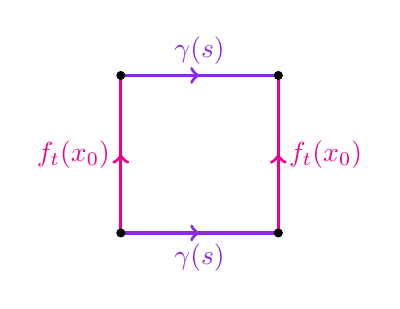
\begin{tikzpicture}[decoration={
		markings,
		mark=at position 0.5 with {\arrow{to}}
	}]
		% Sides as arrows with arrowheads in the middle
		\draw[magenta,very thick,postaction={decorate}] (0,0) -- (0,2) node[midway, left] {$f_t(x_0)$};
		\draw[blue-violet,very thick,postaction={decorate}] (0,2) -- (2,2) node[midway, above] {$\gamma(s)$};
		\draw[magenta,very thick,postaction={decorate}] (2,0) -- (2,2) node[midway, right] {$f_t(x_0)$};
		\draw[blue-violet,very thick,postaction={decorate}] (0,0) -- (2,0) node[midway, below] {$\gamma(s)$};
		
		% Vertices
		\filldraw (2,0) circle (0.05);
		\filldraw (2,2) circle (0.05);
		\filldraw (0,2) circle (0.05);
		\filldraw (0,0) circle (0.05);
	\end{tikzpicture}\]
	Claro, pues $f_0(\gamma(s))=\gamma(s)=f_1(\gamma(s))$, y $f_t(\gamma(0))=f_t(x_0)=f_t(\gamma(1))$. Así es que los bordes de izquierda y arriba representan $f\cdot\gamma$ y los bordes de abajo y derecha $\gamma\cdot f$. Cualquier trayectoria dentro del cuadrado que una la esquina inferior izquierda con la esquina superior derecha representa un camino homotópico a cualquiera de los mencionados.
	\end{proof}

\begin{ejer}
	Use el \hyperref[lema:homotopia]{Lema 1.15} para mostrar que si $X$ se obtiene de un espacio arco-conexo adjuntando una célula $e^n$ con $n\geq2$, entonces la inclusión $A\hookrightarrow X$ induce una función suprayectiva en $\pi_1$.
\end{ejer}
\begin{proof}[Solución]
	El \hyperref[lema:homotopia]{Lema 1.15} nos asegura que si encontramos dos conjuntos abiertos $A_1$ y $A_2$ que contienen al punto base tales que su unión es igual a todo el espacio y su intersección es arco-conexa, entonces cualquier lazo en el espacio se puede ver como el producto de dos lazos, cada uno contenido en un $A_i$.
	
	Tomemos $A_1=e^n$ y $A_2=X-c$, donde $c$ es un punto en el interior de $e^n$. Si escogemos un punto base $x_0$ también en el interior de $e^n$, tenemos las condiciones para el lema. Luego, cualquier lazo en $X$ se puede ver como un lazo solamente en $A_2$, ya que $e^n$ es contraible. Luego, debemos usar el \hyperref[teo:cambioptobase]{teorema de cambio de punto base} para conectar el punto $x_0$ con un $\tilde{x}_0$ que esté en $X\backslash e^n$. Y por último, como $A$ es \hyperref[def:retracto]{retracto por deformación} de $A_2$, sus grupos fundamentales son isomorfos, por lo que podemos pensar que nuestro lazo está en $A$.
\end{proof}
\part{Espacios cubrientes}
\chapter{Espacios cubrientes}
\section{Definición de espacio cubriente}
En la demostración del grupo fundamental del círculo ya habíamos usado la idea de espacio cubriente. Aquí está la definición general:
\begin{defn}
	Un \textbf{espacio cubriente} de $X$ es un espacio $\tilde X$ junto con una función \[p:\tilde X\to X\] tal que cada punto $x\in X$ tiene una vecindad abierta $U\subseteq X$ tal que $p^{-1}(U)$ es una unión disjunta de abiertos de $\tilde X$ de manera que cada uno se proyecta homeomorfamente a $U$ vía $p$.
\end{defn}
\begin{wrapfigure}[13]{l}{0.33\textwidth}
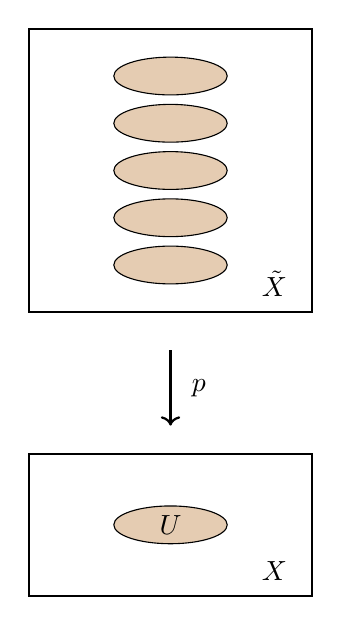
\begin{tikzpicture}[scale=1.2]
	% Rectangle representing X
	\draw[thick] (0,0) rectangle (3,1.5);
	\node at (1.5,0.75) {X};
	
	% Pancake U inside X
	\draw[fill=brown!40] (1.5,0.75) ellipse (0.6 and 0.2);
	\node at (1.5,0.75) {$U$};
	\node at (2.6,0.26) {$X$};
	
	% Rectangle representing \tilde X
	\draw[thick] (0,3) rectangle (3,6);
	\node at (2.6,3.3) {$\tilde{X}$};
	
	% Stacked pancakes above U
	\def\numpans{5}
	\def\pancakeHeight{0.2}
	\def\pancakeSpacing{0.3}
	\def\tildeXtop{6.2}
	
	\foreach \i in {1,...,\numpans} {
		\pgfmathsetmacro\yshift{\tildeXtop - \i*(\pancakeHeight + \pancakeSpacing)}
		\draw[fill=brown!40] (1.5,-0.2+\yshift) ellipse (0.6 and \pancakeHeight);
	}
	 % Arrow from \tilde X to X
	\draw[->, thick] (1.5,2.6) -- (1.5,1.8);
	\node at (1.8,2.2) {$p$};
\end{tikzpicture}
\vspace{-2.6cm}
\end{wrapfigure}
	Introducimos otros términos:
	\begin{itemize}
		\item A la función $p$ le llamamos \textbf{proyección cubriente}.
		\item A $U$ se le llama \textbf{vecindad regular}.
		\item A los abiertos de $p^{-1}(U)$ que se proyectan homeomorfamente a $U$ se les llama \textbf{hojas} de $\tilde X$ sobre $U$.
		\item El conjunto $p^{-1}(x)$ se llama la \textbf{fibra} de $x$ bajo $p$.
	\end{itemize}
	\begin{obs}\leavevmode
		\begin{itemize}
			\item Si $U$ es conexo entonces las hojas de $U$ son las componentes conexas de $p^{-1}$.
			\item El número de hojas sobre $U$ es igual a la cardinalidad de $p^{-1}(x)$.
			\item Este número es \textit{localmente constante}, es decir, es igual para cualquier punto:
		\end{itemize}
	\end{obs}\newpage
	
	\begin{ejems}\leavevmode
		\begin{enumerate}
			\item La identidad $Id:X\to X$.
			\item La proyección natural de la unión disjunta de copias de un espacio, es decir $p:\bigsqcup_{\alpha\in I}X\to X$.
			\item Para cualesquiera dos cubrientes $p:\tilde X\to X$ y $q:\hat X\to X$, la proyección desde la unión disjunta $r:\tilde{X}\sqcup\hat{X}\to X$ definida de la manera natural, también es un cubriente. Esto para decir que nos interesan los cubrientes de espacios conexos cuyos cubrientes sean conexos.
			\item $p:\R\to S^1$ como en la prueba del grupo fundamental del círculo.
			\item Para $n\in\N$, la función	$p:S^1\to S^1$ dada por $p(z)=z^n$
		\end{enumerate}
	\end{ejems}
\section{Levantamiento de homotopía para cubrientes}
\begin{defn}
	Un \textbf{levantamiento} de una función $f:Y\to X$ con respecto a un cubriente $p:\tilde{X}\to X$ es una función $\tilde{f}:Y\to\tilde{X}$ tal que $p\tilde{f}=f$. Es decir, que el siguiente diagrama conmute:
	\[\begin{tikzcd}[column sep=1cm,row sep=1cm]
		&\tilde{X}\arrow[d,"p"]\\
		Y\arrow[ur,dashed,"\tilde{f}"]\arrow[r,swap,"f"]&X
	\end{tikzcd}\]
	\begin{teo}[Propiedad del levantamiento de homotopía para cubrientes]\label{teo-lhc}
		Dado un cubriente $p:\tilde{X}\to X$ y una homotopía $h_t:Y\to X$ y un levantamiento $\tilde{f}_0:Y\to \tilde{X}$ de $f_0$, entonces existe una única homotopía $\tilde{f}_t:Y\to \tilde{X}$ que levanta a cada uno de los $f_t$.
		
		Es decir, que el siguiente diagrama conmuta:
		\[\begin{tikzcd}[column sep=1cm,row sep=1cm]
			Y\times\{0\}\arrow[r,"\tilde{f}_0"]\arrow[rd,"f_0" near end]\arrow[d,hook]&\tilde{X}\arrow[d,"p"]\\
			Y\times I\arrow[r]\arrow[ru,dashed]&X
		\end{tikzcd}\]
	\end{teo}
\end{defn}
\section{El homomorfismo inducido de la proyección cubriente}
Dada una proyección cubriente $p:\tilde{X}\to X$, ¿qué propiedades tendrá el mapeo inducido $p_*:\pi_1(\tilde{X},\tilde{x}_0)\to (X,x_0)$ donde $p(\tilde{x}_0)=x_0$. Resultará que es inyectivo.

Para demostrar esto, se usará la \hyperref[teo-lhc]{Propiedad del levantamiento de homotopía para cubrientes}. Entonces primero vamos a ver un par de casos sencillos de cómo se usa este teorema:
\begin{prop}[Propiedad del levantamiento de caminos]
	Un camino tiene un único levantamiento una vez definido a dónde va a dar el punto inicial. Para verlo, escogemos el caso en que $Y$ consta de un sólo punto, así que una homotopía de $Y\times I$ es un camino en $X$.
\end{prop}
\begin{obs}
	El levantamiento de un camino constante es un camino constante.
\end{obs}
\begin{obs}
	Si $Y=I$, y $H:I\times I$ es una homotopía $\rel 0,1$, entonces el levantamiento $\tilde{H}$ también es una homotopía $\rel 0,1$.
\end{obs}
Ahora sí,
\begin{prop}
	Dada una proyección cubriente $p:\tilde{X}\to X$, el mapeo inducido $p_*:\pi_1(\tilde{X},\tilde{x}_0)\to (X,x_0)$ es inyectivo. Más aún, $p_*\left(\pi_1(\tilde{X},\tilde{x}_0)\right)\leq\pi_1(X,x_0)$ consiste de los lazos basados en $x_0$ que se levantan a lazos en $\tilde{X}$ basados en $\tilde{x}_0$.
\end{prop}
\section{El número de hojas de un cubriente y el grupo fundamental}
\begin{prop}
	Sea $p:\tilde{X}\to X$ un cubriente con $\tilde{X}$ y $X$ conexos por trayectorias. Entonces el número de hojas del cubriente es igual al índice de $p_*(\pi_1(\tilde{X},\tilde{x}_0))$ en $\pi_1(X,x_0)$.
\end{prop}
\section{El criterio de levantamiento de funciones}
Consideremos un cubriente $p:\tilde{X}\to X$ y una función cualquiera $f:Y\to X$. ¿Bajo qué condiciones será posible levantar esta función al cubriente? Queremos que este diagrama conmute:
\[\begin{tikzcd}[column sep=1cm,row sep=1cm]
	&\tilde{X}\arrow[d,"p"]\\
	Y\arrow[ur,dashed,"\tilde{f}"]\arrow[r,swap,"f"]&X
\end{tikzcd}\]
Estas funciones no siempre van a existir. Para saber cuándo sí, primero veamos:
\begin{defn}
	Decimos que un espacio topológico $Y$ es \textbf{localmente arco-conexo} si para todo punto $y\in Y$ y cada vecindad $U$ de $y$, existe $y\in V\subseteq U$ que es arcoconexa.
\end{defn}
\begin{prop}
	Sean $p:(\tilde{X},\tilde{x}_0)\to (X,x_0)$ un cubriente y una función $f:(Y,y_0)\to (X,x_0)$ con $Y$ espacio arco-conexo y localmente arco-conexo. Entonces existe un levantamiento $\tilde{f}:(Y,y_0)\to(\tilde{X},x_0)$ si y sólo si $f_*\pi_1(Y,y_0)\subseteq p_*\pi_1(\tilde{X},\tilde{x}_0)$.
\end{prop}
\section{Unicidad del levantamiento de funciones}
	¿Bajo qué condiciones un levantamiento es único? Cuando dos levantamientos coincidan en un punto, tienen que ser iguales. (Siempre que el dominio sea arco-conexo.)
	
	\begin{prop}
		Sean $p:\tilde{X}\to X$ un cubriente y $f:Y\to X$ una función. Si dos levantamientos $\tilde{f}_1,\tilde{f}_2:Y\to\tilde{X}$ de $f$ coinciden en un punto y $Y$ es conexo, entonces $\tilde{f}_1=\tilde{f}_2$.
		\[\begin{tikzcd}
				&\tilde{X}\arrow[d,"p"]\\
				Y\arrow[ru,"\tilde{f}_1"]\arrow[ru,swap,"\tilde{f}_2"]\arrow[r,swap,"f"]&X
			\end{tikzcd}\]
	\end{prop}



% Aquí está la prop como estaba en el video, pero me fui por la versión de Hatcher	

%\begin{prop}
%	Sean $p:(\tilde{X},\tilde{x}_0)\to (X,x_0)$ un cubriente y $f:(Y,y_0)\to (X,x_0)$ una función. Si $\tilde{f}_1,\tilde{f}_2:Y\to\tilde{X}$ son levantamientos de $f$ que coinciden en un punto y $Y$ es conexo, entonces $\tilde{f}_1=\tilde{f}_2$.
%	\[\begin{tikzcd}
%		&(\tilde{X},\tilde{x_0})\arrow[d,"p"]\\
%		(Y,y,_0)\arrow[ru,"\tilde{f}_1"]\arrow[ru,swap,"\tilde{f}_2"]\arrow[r,swap,"f"]&(X,x_0)
%	\end{tikzcd}\]
%\end{prop}
\section{El cubriente universal}
En esta sección intentaremos clasificar todos los cubrientes que puede tener un espacio. La primera pregunta que nos hacemos en qué casos un cubriente tiene un cubriente cuyo grupo fundamental sea trivial. Tal cubriente será llamado el \textbf{cubriente universal}, que será universal en cuanto a que va a cubrir a cualquier otro cubriente.

Supongamos que tenemos un espacio $X$ que
\begin{itemize}
	\item es arco-conexo.
	\item es localmente arco-conexo.
\end{itemize}
Ahora tomemos un cubriente $p:\tilde{X}\to X$ como decíamos, simplemente conexo. Cuando tomamos un punto $p\in X$ y una vecindad regular, cualquier lazo contenido en esa vecindad, podemos levantarlo a una de sus preimágenes. Pero como el cubriente $\tilde{X}$ es simplemente conexo, entonces el lazo levantado es contraible, y esa homotopía se proyecta a una homotopía del lazo con el que empezamos al lazo constante.

\begin{defn}
	Un espacio es \textbf{semilocalmente simplemente conexo} si para cada $x\in X$ existe una vecindad $U$ tal que todo lazo contenido en $U$ se retrae al lazo constante $c_x$ en $X$. Equivalenetemente, el homomorfismo inducido por la inclusión $\pi_1(U,x_0)\to(X,x_0)$ es constante.
\end{defn}
O sea que ya demostramos que si $X$ tiene cubriente universal entonces es semilocalmente simplemente conexo. Ahora queremos ver que el regreso también es cierto (cuando $X$ también es arco-conexo y localmente arco-conexo).
\begin{prop}
	Un espacio $Y$ es simplemente conexo si y sólo si para todo $x,y\in Y$ existe una única clase de homotopía $\rel0,1$ de caminos que unen $x$ a $y$.
	
	Esto implica que hay una biyección entre los puntos de $Y$ y las clases de equivalencia de caminos que empiezan en $x_0$, es decir, $Y\leftrightarrow \{[\gamma]:\gamma(0)=x_0\}$.
	
	Ahora consideremos un cubriente $p:\tilde{X}\to X$ con $\tilde{X}$ simplemente conexo y un punto $\tilde{x}\in\tilde{X}$. Denotemos $p(\tilde{x}_0)=x_0\in X$. Entonces, por lo dicho hace un momento los puntos en el espacio cubriente $\tilde{X}$ están in biyección con los caminos que empiezan en $\tilde{x}$, y proyectando mediante $p$, vamos a dar a los caminos que comienzan en $x_0$. Usando la propiedad del levantamiento de homotopía, se verifica que esa correspondencia es biyectiva: \[\{[\gamma]:\gamma(0)=\tilde{x}_0\}\leftrightarrow\{[\beta]:\beta(0)=x_0\}\]
\end{prop}
Ahora sí:
\begin{teo}
	Supongamos que $X$ es un espacio topológico arco-conexo, localmente arco-conexo y semilocalmente simplemente conexo, y tomemos un punto base $x_0\in X$. El espacio \[\tilde{X}:=\{[\gamma]:\gamma(0)=x_0\}\]
	acompañado de la función
	\begin{align*}
		p:\tilde{X}&\to X\\
		[\gamma]&\mapsto\gamma(1)
	\end{align*}
	son un cubriente universal de $X$. Es decir:
	\begin{itemize}
		\item $\tilde{X}$ tiene una topología.
		\item $p$ es continua.
		\item $p$ es cubriente.
		\item $\tilde{X}$ es simplemente conexo.
	\end{itemize}
\end{teo}
\section{El teorema de clasificación de cubrientes}
En esta sección veremos, grosso modo, que hay una correspondencia entre cubrientes universales (salvo isomorfismo) con los subgrupos del grupo fundamental.

\begin{prop}
	Sea $X$ un espacio topológico arco-conexo, localmente arco-conexo y semilocalmente simplemente conexo. Entonces para todo $H\leq\pi_1(X,x_0)$ existe un cubriente $p:X_H\to X$ tal que $p_{*}\left(\pi_1(X_H,\tilde{x}_0)\right)=H$.
\end{prop}
\begin{proof}
	Usando la construcción del cubriente universal, tomamos una relación de equivalencia determinada por $H$ y proponemos el espacio cociente $\tilde{X}/\sim{}$.
\end{proof}
Ahora nos preguntamos si este cubriente es único de alguna manera. La respuesta es que sí, pero primero debemos definir la noción de isomorfismo de cubrientes.
\begin{defn}
	Dos cubrientes $\tilde{X}_1$ y $\tilde{X}_2$ son \textbf{isomorfos} si existe un homeomorfismo que hace conmutar el siguiente diagrama:
	\[\begin{tikzcd}
		\tilde{X}_1\arrow[dr,swap,"p_1"]\arrow[rr,"homeo"]&&\tilde{X}_2\arrow[dl,"p_2"]\\
		&X
	\end{tikzcd}\]
\end{defn}
\begin{prop}
	Si $X$ es arco-conexo y localmente arco-conexo, entonces $p_1:\tilde{X}_1\to X$ y $p_2:\tilde{X}_2\to X$ son isomorfos mediante $f:\tilde{X}_1\to\tilde{X}_2$, con ciertos puntos base tales que $f(\tilde{x}_1)=\tilde{x}_2$ y $p_1(\tilde{x}_1)=p_2(\tilde{x}_2)=x_0\in X$ si y sólo si
	\[p_{1*}\left(\pi_1(\tilde{X}_1,\tilde{x}_1)\right)=p_{2*}\left(\pi_2(\tilde{X}_2,\tilde{x}_2)\right)\]
\end{prop}
Notemos que en la proposición anterior, $p_{1*}\left(\pi_1(\tilde{X}_1,\tilde{x}_1)\right)=H$ era un subgrupo arbitrario de $\pi_1(X,x_0)$. Hemos demostrado que dos cubrientes que provienen del mismo grupo son isomorfmos. De hecho, ya demostramos:

\begin{teo}
	Sean $X$ un espacio conexo, localmente arco-conexo y semilocalmente arco-conexo, y $x_0\in X$. Entonces la correspondencia
	\[
	\begin{array}{c}
		\{p:(\tilde{X},\tilde{x}_0)\to(X,x_0):p\text{ es un cubriente}\}\Big/\text{isomorfismo}\\\leavevmode\\
		\tilde{X}\xrightarrow{p} X
	\end{array}
	\begin{array}{c}
		\longleftrightarrow\\\leavevmode\\
		\mapsto
	\end{array}
	\begin{array}{c}
		\{H\leq\pi_1(X,x_0)\}\\\leavevmode\\
		p_*\left(\pi_1(\tilde{X},\tilde{x}_0)\right)
	\end{array}
	\]
	es una biyectiva.
\end{teo}
Notemos que si cambiamos la elección del punto base $\tilde{x}_0$ en el cubriente, podemos ir a dar a un subgrupo muy diferente. Esto nos lleva a:
\begin{teo}
	Sean $X$ un espacio conexo, localmente arco-conexo y semilocalmente arco-conexo, y $x_0\in X$. Entonces hay una biyección
		\[
	\begin{array}{c}
		\{p:\tilde{X}\to X:p\text{ es un cubriente}\}\Big/\text{isomorfismo}\\\leavevmode\\
		\tilde{X}\xrightarrow{p} X\\
		\text{escojo }\tilde{x}_0\in p^{-1}(x_0)
	\end{array}
	\begin{array}{c}
		\longleftrightarrow\\\leavevmode\\
		\mapsto
	\end{array}
	\begin{array}{c}
		\{H\leq\pi_1(X,x_0)\}\Big/\text{conjugación}\\\leavevmode\\
		p_*\left(\pi_1(\tilde{X},\tilde{x}_0)\right)
	\end{array}
	\]
\end{teo}

\section{Transfromaciones de cubierta}
	\begin{defn}
		Tomemos un espacio $X$ y algún cubriente $p:\tilde{X}\to X$. Una \textbf{transformación de cubierta} es un isomorfismo de $\tilde{X}$ en sí mismo, es decir, homeomorfismos que hacen conmutar este diagrama:
		\[\begin{tikzcd}
			\tilde{X}\arrow[r,"f"]\arrow[d,swap,"p"]&\tilde{X}\arrow[dl,"p"]\\
			X
		\end{tikzcd}\]
		Es decir, $pf=p$
	\end{defn}
		El conjunto $G(\tilde{X}):=\left\{f:\tilde{X}\to\tilde{X}:f\text{ es transformación de cubierta}\right\}$ tiene estructura de grupo, y le llamaremos \textbf{el grupo de transformaciones de cubierta}.
	\begin{ejem}
		El cubriente $f_n:S^1\to S^1$ dado por $z\mapsto z^n$ tiene grupo de transformaciones de cubierta $G(f_n:S^1\to S^1)=\Z/n\Z$. Además, $f_{n*}\pi_1(S^1)=n\Z$. O sea que $G(f_n:S^1\to S^1)\cong\pi_1(S^1)/f_{n*}\pi_1(S^1)$. Y esto no es ninguna casualidad.
		
		Además, para el cubriente universal de $S^1$, que es $\exp:\R\to S^1$ también se cumple, ya que el grupo fundamental es trivial, es decir, $G(\exp:\R\to S^1)\cong\Z/\{0\}\cong\Z$.
	\end{ejem}
	\begin{prop}
		Si $g,f:\tilde{X}\to\tilde{X}$ son transformaciones de cubierta con $\tilde{X}$ arco-conexo y tales que existe $x\in\tilde{X}$ con $g(x)=f(x)$, entonces $g=f$.
	\end{prop}
	\begin{proof}
		Basta pensar que la transformación de cubierta es un levantamiento de la proyección cubriente:
		\[\begin{tikzcd}
			&\tilde{X}\arrow[d,"p"]\\
			\tilde{X}\arrow[ur,dashed,"f"]\arrow[r,"p"]&X
		\end{tikzcd}\]
		Por el teorema del levantamiento de funciones, $f$ es único una vez que escogemos un punto $y\in f^{-1}(x)$ en la fibra de $x$.
	\end{proof}
	\begin{defn}
		Decimos que un cubriente $p:\tilde{X}\to X$ es \textbf{normal} si para cualquier $x\in X$ y $\tilde{x},\tilde{x}'\in\tilde{X}$ existe una transformación de cubierta $f:\tilde{X}\to\tilde{X}$ tal que $f(\tilde{x})=\tilde{x}'$. Es decir, que el grupo de transformaciones de cubierta actúa transitivamente en las fibras.
	\end{defn}
	\begin{prop}
		Sea $p:(\tilde{X},\tilde{x}_0)\to (X,x_0)$ un cubriente con $\tilde{X}$ y $X$ arco-conexo y localmente arco-conexo. Sea $H=p_*\pi_1(\tilde{X},\tilde{x}_0)\leq\pi_1(X,x_0)$. Entonces
		\begin{enumerate}[label=\alph*)]
			\item El cubriente es normal si y sólo si $H\trianglelefteq\pi_1(X,x_0)$.
			\item $G(\tilde{X})\cong N(H)/H$
			donde $N(H)=\left\{g\in\pi_1(X,x_0)|g^{-1}Hg=H)\right\}$
		\end{enumerate}
		En particular, cuando $\tilde{X}$ es normal, $G(\tilde{X})\cong\pi_1(X,x_0)/H$. Y si además $\tilde{X}$ es el cubriente universal, simplemente tenemos que $G(\tilde{X})\cong\pi_(X,x_0)$.
	\end{prop}
\section{Acciones de grupos y cubrientes}\label{sec:acciones}
\begin{defn}
	Decimos que un grupo $G$ \textbf{actúa} en $X$ si hay un homomorfismo de grupos
	\begin{align*}
		\varphi:G\to\text{Homeo}(X)\\
		g\mapsto\varphi(g):X\to &X\\
		x\mapsto&\varphi(g)(x)
	\end{align*}
	de forma que
	\begin{itemize}
		\item  $\varphi(g_1g_2)=\varphi(g_1)\varphi(g_2)$
		\item $(g_1g_2)x=g_1(g_2(x))$
		\item $\varphi(1_G)=Id_X$
	\end{itemize}
	Y se denota $G\curvearrowright X$.
	La \textbf{órbita} de un punto $x\in X$ es el conjunto $\Orb\{g(x):g\in G)\}$.
\end{defn}
Notemos que la relación $x\sim{}y\iff y\in\Orb(x)$ es de equivalencia, así que podemos pensar en el espacio cociente $X/\sim{}:=X/G$. Nos hacemos la siguiente pregunta: dada una acción de grupos $G\curvearrowright Y$, ¿cuándo $Y/G$ es un cubriente?
\begin{defn}
	Decimos que $G\curvearrowright Y$ es una \textbf{acción cubriente} si se cumple cualquiera de los dos siguientes condiciones equivalentes:
	\begin{itemize}
		\item Cualquier punto $y\in Y$ tiene una vecindad $U$ tal que $(g_1U\cap g_2U)\neq\emptyset\implies g_1=g_2$
		\item Cualquier punto $y\in Y$ tiene una vecindad $U$ tal que $gU\cap U\neq\emptyset\implies g=1_G$.
	\end{itemize}
	En particular, estas condiciones implican que la acción es \textbf{libre}, es decir, que si $g(y)=y$ para cualesquiera $g\in G$ y $y\in Y$, entonces, $g=1_G$.
\end{defn}
\begin{prop}
	Dada una acción cubriente $G\curvearrowright Y$,
	\begin{enumerate}[label=\alph*)]
		\item La proyección cociente $p:Y\to Y/G$ dada por $p(y)=Gy$ es un cubriente normal.
		\item Si $Y$ es arco-conexo, $G$ es el grupo de transformaciones de cubierta de $p$.
		\item Si $Y$ es arco-conexo y localmente arco-conexo, $G\cong\pi_1(Y/G,y_0)/p_*\pi_1(Y,\tilde{y}_0)$
	\end{enumerate}
\end{prop}
\begin{coro}
	Si además $Y$ es simplemente conexo, por b) y por c), $G=G(\tilde{Y})\cong\pi_1(Y/G,y_0)$.
\end{coro}
\chapter{Ejercicios}
\begin{ejer}
	\textbf{Sean $S$ la 2-esfera y $T$ el 2-toro. Calcule el grupo fundamental $G$ de $X := S \vee T$, construya el cubriente universal $\widetilde{X} \to X$ y describa la acción por transformaciones de cubierta de $G$ en $\widetilde{X}$.}
	\begin{proof}[Solución] Por el teorema de Van Kampen, $\pi_1(S\vee T,x_0)=\Z\times\Z$. El cubriente universal es $\R^2$ con copias de $S^2$ pegadas en cada punto con coordenadas enteras, y la acción por transformaciones de cubierta es justamente la colección de traslaciones por vectores con coordenadas enteras.
	\end{proof}
\end{ejer}
\begin{ejer}
	\textbf{Sea $f:X\to Y$ un cubriente. Muestre que si $Y$ es un espacio CW, entonces $X$ también.}
\end{ejer}
\begin{proof}[Solución]
	Primero definamos $X^0:=f^{-1}(Y^0)$. La idea es usar el teorema de levantamiento de funciones para las funciones de pegado. Sin embargo, esto no se puede hacer para construir el 1-esqueleto de $X$, porque $S^0$ no es conexo. Lo que sí podemos hacer es tomar la función característica:
		\[\begin{tikzcd}
		&X\arrow[d,"f"]\\
		D_\alpha^1\arrow[ru,dashed,"\tilde{\Phi}_\alpha"]\arrow[r,swap,"\Phi_\alpha"]&Y^1
	\end{tikzcd}\]
	que se levanta porque $D^1_\alpha$ es contraible. Con esto podemos definir la función de pegado $\tilde{\varphi}_\alpha:S^0\to X^0$ directamente como $\tilde{\varphi}_\alpha(-1)=\tilde{\Phi}_\alpha(0)$ y $\tilde{\varphi}_\alpha(1)=\tilde{\Phi}_\alpha(1)$ que funciona bien porque la función característica extiende a la función de pegado.
	
	El mismo método funciona para construir el 2-esqueleto, y las demás funciones de pegado se pueden levantar directamente porque $S^n$ es simplemente conexo para $n>1$.
	
	Si $Y$ es de dimensión finita, sabemos que $Y=Y^n$. *Falta un poquito*
\end{proof}
\begin{ejer}
	\textbf{Demuestre que para todo $g\geq2$ existe un cubriente $S_g\to S_2$, es decir, que toda superficie de género 2 es cubierta por cualquier superficie de género $g\geq 2$. Demuestre además que el toro no es cubierto por ninguna superficie cerrada de género $g\geq2$.}
\end{ejer}
\begin{proof}
	Aquí debemos visualizar $S_g$ como una dona-flor con un agujero en el centro y $g-1$ pétalos. En este caso, el grupo cíclico de $g-1$ es una acción cubriente en $S_{g}$ rotando alrededor del hoyo del centro. El espacio cociente resultante es justamente $S_2$, ya que se identifican todos los pétalos.
	
	Supongamos que existe un cubriente $p:S_g\to T$ con $g\geq2$. Sabemos que el homomorfismo inducido $p_*$ es inyectivo, por lo que $p_*\pi_1(S_g)\approx\pi_1(S_g)$, que, por el teorema de Van Kampen sabemos que es de la forma $\langle a_1,b_1,\ldots,a_g,b_g|a_1b_1a_1^{-1}b_1^{-1}\ldots a_{g}b_ga_g^{-1}b_g^{-1}\rangle$ que no es conmutativo. Pero cualquier subgrupo de $\pi_1(T)\approx\Z\times\Z$ es conmutativo.
\end{proof}
\begin{ejer}[Hatcher, 1.3.8]
	\textbf{Sean $\tilde{X}$ y $\tilde{Y}$ espacios cubrientes simplemente conexos de espacios arco-conexos y simplemente conexos $X$ y $Y$. Muestre que si $X\simeq Y$, entonces $\tilde{X}\simeq\tilde{Y}$. (Quizás convenga usar el ejercicio \hyperref[hatcher:0.11]{0.11, Hatcher})}
\end{ejer}
\begin{proof}[Solución]
	Todo está en el siguiente diagrama conmutativo:
	\[\begin{tikzcd}
		&&&\tilde{X}\arrow[dd,"p"]\\
		&&\tilde{Y}\arrow[d,"q"]\arrow[ru,dashed,"\tilde{g}"]\\
		\tilde{X}\arrow[rru,dashed,"\tilde{f}"]\arrow[r,swap,"p"]&X\arrow[r,swap,"f"]&Y\arrow[r,swap,"g"]&X
	\end{tikzcd}\]
	Donde:
	\begin{enumerate}
		\item $f$ y $g$ son equivalencias homotópicas entre $X$ y $Y$.
		\item $pf$ se levanta a una única función $\tilde{f}$ por las hipótesis de conexidad. Lo mismo para encontrar $\tilde{g}$.
		\item Como todo conmuta, $\tilde{g}\tilde{f}$ es un levantamiento de $gfp$.
		\item Como $gf\simeq Id_X$, entonces $gfp\simeq p$. Esta homotopía se levanta de manera única a una homotopía $H:\tilde{X}\times I\to\tilde{X}$ ya que, como acabamos de ver, $H(\underline{\hspace{5pt}},0)=\tilde{g}\tilde{f}$. Luego, $pH(\underline{\hspace{5pt}},1)=p$.
		\item Así que $H(\underline{\hspace{5pt}},1):=h$ es un levantamiento de $p$, igual que la identidad. Si lográramos ver que coinciden en un sólo punto, es decir que $h$ fija a cualquier punto, por unicidad del levantamiento de funciones, tendríamos que $h=Id_{\tilde{X}}$.
		
		Pero no tenemos certeza de que eso ocurre. Lo que sí sabemos que como $\tilde{X}$ es simplemente conexo, entonces $p$ es un cubriente normal. O sea que el grupo de transformaciones de cubierta actúa transitivamente en las fibras de los puntos.
		
		Entonces tomemos un punto $\xi\in\tilde{X}$. Si $h$ no lo fija, ni modo, pero sabemos que existe una transformación de cubierta $u$ tal que $u(h(\xi))=\xi$.
		
		Ahora sí, por unicidad del levantamiento de funciones, $uh= Id_{\tilde{X}}$.
		\item Entonces $u\tilde{g}\tilde{f}\simeq Id_{\tilde{X}}$.
		\item El \hyperref[hatcher:0.11]{ ejercicio 0.11}, nos asegura que si encontramos dos funciones $\phi,\psi:\tilde{X}\to\tilde{X}$ tales que $\phi\tilde{f}\simeq Id_{\tilde{X}}$ y $\tilde{f}\psi\simeq Id_{\tilde{Y}}$, entonces $\tilde{f}$ es una equivalencia homotópica y terminamos. Ya encomtramos $\phi$.
		
		Para encontrar $\psi$, simplemente hacemos el mismo razonamiento sólo que ahora necesitamos una transformación de cubierta $w$ tal que $\tilde{f}\tilde{g}w\simeq Id_{\tilde{Y}}$.
		
		Es decir, aquí hay que aplicar la $w$ antes de la función que obtenemos mediante la homotopía, digamos $\bar{h}$. Esto es legal: en vez de mover a $\bar{h}(\xi)$ de regreso a $\xi$, de antemano movemos a $\xi$ mediante $w$ a un punto en la preimagen de $\xi$ bajo $\bar{h}$. Aunque quizás $\bar{h}$ no es suprayectiva, basta con escoger $\xi\in\img\bar{h}$.
	\end{enumerate}
\end{proof}
\begin{ejer}
	Demuestre que si $X$ es arco-conexo y localmente arco-conexo y $\pi_1(X)$ es finito, entonces toda función $f:X\to S^1$ es homotópica a una constante.
\end{ejer}
\begin{proof}
	Como $\pi_1(X)$ es finito y $f_*\pi_1(X)$ es un subgrupo de $\pi_1(S^1)\approx\Z$, y el único subgrupo finito de $\Z$ es el trivial, tenemos que $f_*\pi_1(X)\approx0$. Luego, existe un levantamiento $\tilde{f}:X\to\R$ al cubriente universal del círculo:
	\[\begin{tikzcd}
		&\R\arrow[d,"p"]\\
		X\arrow[ur,dashed,"\tilde{f}"]\arrow[r,swap,"f"]&S^1
	\end{tikzcd}\]
	Como $X$ es arco-conexo, su imagen debe ser un intervalo, que es contraible, es decir, $\img\tilde{f}\simeq\{\tilde{x}_o\}$ vía una equivalencia homotópica $\phi:\img\tilde{f}\to\{\tilde{x}_0\}$ y $\psi:\{\tilde{x}_0\}\to\img\tilde{f}$. Desde luego, estas dos funciones no son más que la constante $\tilde{x}_0$, así que en realidad tenemos una homotopía $id_{\img\tilde{f}}\simeq\tilde{x}_0$, digamos $h:\img\tilde{f}\times I\to \img\tilde{f}$ tal que $h(x,0)=x$ y $h(x,1)=\tilde{x}_0$.
	
	La función $g=p\circ h\circ\tilde{f}$ es una homotopía entre $f=p\circ\tilde{f}$ y la constante $x_0=p(\tilde{x}_0)$.
\end{proof}
\part{Homología}
\chapter{Álgebra Homológica}
\section{Conceptos básicos}
	En este capítulo $R$ denotará un anillo asociativo con unidad (no necesariamente conmutativo). Normalmente pensaremos que es alguno de los siguientes: $\Z, \Q, \R$.
	
	Recordemos que un $R$-módulo es básicamente un espacio vectorial pero los escalares están $R$.
	\begin{defn}
		Un \textbf{$R$-complejo de cadenas} es una sucesión de $R$-módulos y homomorfismos
		\[\begin{tikzcd}
			(C_\bullet,\partial):= \quad \cdots \arrow{r} & C_p \arrow{r}{\partial_p} & C_{p-1} \arrow{r}{\partial_{p-1}} & C_{p-2} \arrow{r} & \cdots
		\end{tikzcd}\]
		tal que $\partial_{p-1}\partial_p=0$ para toda $p\in \mathbb{Z}$, que es equivalente a que $\text{img }\partial_p\subseteq\ker{\partial_{p-1}}$.
	\end{defn}
	
	\begin{defn}
		Un \textbf{morfismo de $R$-complejos de cadenas} es $(C_\bullet{},\partial)\to(D_\bullet{},\delta)$ es una sucesión de $R$-homomorfismos $C_p\xrightarrow[]{f_p} D_p$ tal que el siguiente diagrama conmuta:
		\[
		\begin{tikzcd}
			\cdots \arrow{r} & C_{p+1} \arrow{r}{\partial_{p+1}} \arrow{d}{f_{p+1}} & C_p \arrow{r}{\partial_p} \arrow{d}{f_p} & C_{p-1} \arrow{r} \arrow{d}{f_{p-1}} & \cdots \\
			\cdots \arrow{r} & D_{p+1} \arrow{r}{\delta_p} & D_p \arrow{r}{\delta_p} & D_{p-1} \arrow{r} & \cdots
		\end{tikzcd}
		\]
		es decir $f_{p-1}\partial_p=\delta_pf_p$ para toda $p\in\mathbb{Z}$.
	\end{defn}
	\begin{defn}
		Decimos que $(D_\bullet,\delta)$ es un \textbf{subcomplejo de cadenas} de $(C_\bullet,\partial)$ si $D_p\leq C_p$ para toda $p\in\mathbb Z$ y $\partial|_{D_p}=\delta_p$. El cociente $(C_\bullet/D_\bullet,\partial)$ es el complejo de cadenas dado por
		\[
		\begin{tikzcd}
			\cdots \arrow{r} & C_{p+1}/D_{p+1} \arrow{r}{\partial_{p+1}} & C_{p}/D_{p} \arrow{r}{\partial_{p}} & C_{p-1}/D_{p-1} \arrow{r} & \cdots
		\end{tikzcd}
		\]
		donde los mapeos frontera son de la forma $\partial_p/\delta_p([c])=[\partial_p(c)]$.
	\end{defn}
	\begin{defn}\leavevmode
		\begin{itemize}
			\item Los elementos en $C_p$ se llaman \textbf{cadenas de dimensión $p$}.
			\item Los elementos en $\ker\partial_p:=Z_p$ se llaman \textbf{ciclos de dimensión $p$}.
			\item Los elementos en $\text{img }\partial_{p+1}:=F_p:=B_p$ se llaman \textbf{fronteras de dimensión $p$}.
		\end{itemize}
	\end{defn}
	
	\begin{defn}
		El \textbf{$p$-ésimo grupo de homogía} de $(C_{\bullet{}},d)$ es
		\[H_p(C_{\dot{}}):=Z_p/B_p=\ker\partial_p/\text{img }\partial_{p+1}\]
		Y decimos que dos ciclos $c$ y $c'$ son \textbf{homólogos} si $[c]=[c']\in H_p(C_\bullet)$.
	\end{defn}
	Veamos una figura de dos ciclos homólogos:
	\begin{figure}[H]
		\centering
		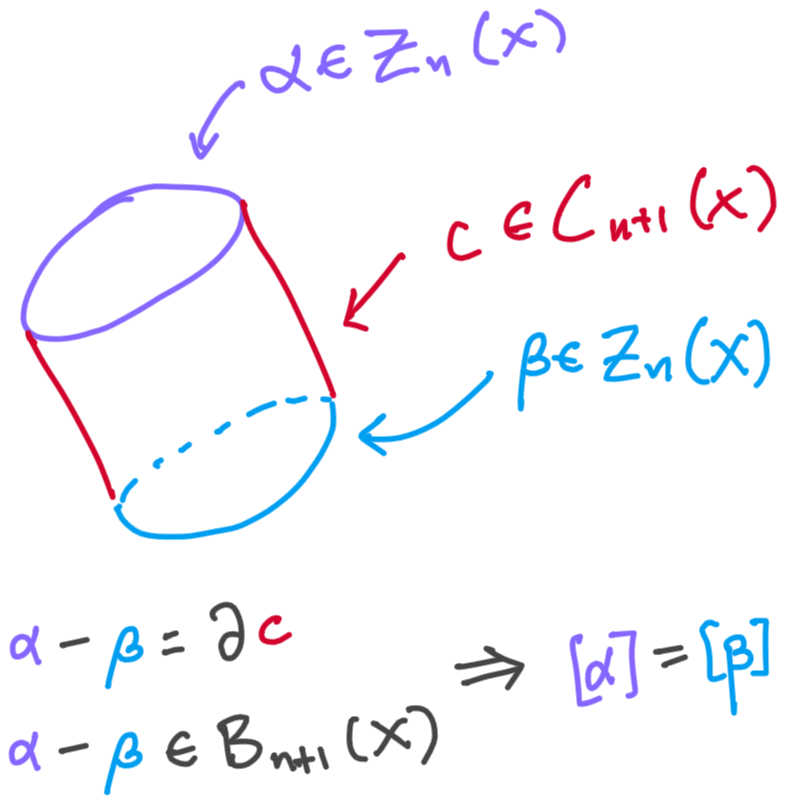
\includegraphics[width=0.4\linewidth]{Homología/H1.png}
	\end{figure}
	\begin{ejer}[Función inducida]
		Si $(C_\bullet{},\partial)\xrightarrow f(C'_\bullet{},\partial')$ es un homeomorfismo, entonces $f(Z_p)\subseteq Z'_p$ y $f(B_p)\subseteq B'_p$ así que la función inducida
		\begin{align*}
			\bar f_p:H_p(C_\bullet{})\to & H_p(C_\bullet{})\\
			a+B_p\mapsto& f_p(a)+B'_p
		\end{align*}
		está bien definida.
		Si además tenemos un segundo homomorfismo $(C'_\bullet,\partial')\xrightarrow{g}(C''_\bullet,\partial'')$, entonces $\overline{g\circ f}=\bar g\circ\bar f$. Y por último, $\overline{Id}_{C_p}=Id_{H_p(C)}$.
	\end{ejer}
	Con este ejercicio comenzamos a ver las propiedades funtoriales de la homología, aunque por ahora no profundizaremos en este lenguaje.
	\section{Sucesiones exactas}
	\begin{defn}
		Decimos que la sucesión 
		\[
		\begin{tikzcd}[column sep=small]
			\cdots \arrow{r} & C_p \arrow{r}{f_p} & C_{p-1} \arrow{r}{f_{p-1}} & C_{p-2} \arrow{r} & \cdots
		\end{tikzcd}
		\]
		es \textbf{exacta en $C_p$} si  $\text{img }f_p=\ker{f_{p-1}}$. Y la sucesión es \textbf{exacta} si es exacta en todos los $C_p$. Esto sucede si y sólo si $H_p(C_\bullet{})=0$ para todo $p\in\mathbb{Z}$.
	\end{defn}
	\begin{obs}\leavevmode
		\begin{itemize}
			\item El grupo de homología mide qué tan lejos está la sucesión de ser exacta.
			\item La sucesión puede ser "finita", o sea pueden haber muchos módulos que son cero.
		\end{itemize}
	\end{obs}
	\begin{defn}
		Una sucesión exacta de la forma \[0\to P\to Q\to R\to 0\] se llama \textbf{sucesión exacta corta}. Las sucesiones exactas infinitas en ambas direcciones se llaman \textbf{sucesiones exactas largas}.
	\end{defn}
	\begin{prop}\label{sucex}\leavevmode
		\begin{enumerate}
			\item $0\to A\xrightarrow{\alpha}B$ es exacta si y sólo si $\ker{\alpha}=0$, es decir $\alpha $ es inyectiva.
			\item $A\xrightarrow{\alpha}B\to 0$ es exacta si y sólo si $\text{img }{\alpha}=B$, es decir $\alpha $ es suprayectiva.
			\item $0\to A\xrightarrow{\alpha}B\to 0$ es exacta si y sólo si $\alpha $ es un isomorfismo por los dos incisos anteriores.
			\item $0\to A\xrightarrow{\alpha}B\xrightarrow{\beta} C\to0$ es exacta si y sólo si $\alpha$ es inyectiva, $\beta$ es suprayectiva y $\ker\beta=\text{img }\alpha$, de manera que $\beta$ induce un isomorfismo $C\cong B/\text{img }\alpha$.
			
			Si pensamos que $\alpha$ es la inclusión de $A$ como subgrupo de $B$, podemos escribir $C\cong B/A$ .
		\end{enumerate}
	\end{prop}
	\begin{obs}[Primer teorema de isomorfismo] Si $M'\subseteq M$, entonces
		\[
		\begin{tikzcd}
			0 \arrow{r} & M' \arrow[hookrightarrow]{r} & M \arrow[twoheadrightarrow]{r} & M/M' \arrow{r} & 0
		\end{tikzcd}
		\]
		es una sucesión exacta.
	\end{obs}
	\section{Homotopía}
	\begin{defn}
		Dos homomorfismos 
		\begin{align*}
			f,g:(C_\bullet,\partial)\to(C'_\bullet,\partial')
		\end{align*}
		son \textbf{homotópicos} si existen homomorfismos $H_p:C_p\to C'_{p+1}$ para toda $p\in\Z$ tales que \[f_p-g_p=\partial'_{p+1}H_p+H_{p-1}\partial_p\] Estas flechas se pueden visualizar aquí:
		\[\begin{tikzcd}[column sep=large, row sep=large]
			\cdots \arrow{r} & C_{p+1} \arrow{r}{\partial_{p+1}} \arrow{d}[left]{f_{p+1}-g_{p+1}} & C_p \arrow{r}[blue]{\partial_p} \arrow{d}[right,red]{f_p-g_p} \arrow{ld}[left,blue]{H_p} & C_{p-1} \arrow{r} \arrow{d}[right]{f_{p-1}-g_{p-1}} \arrow{ld}[right,blue]{H_{p-1}} & \cdots \\
			\cdots \arrow{r} & C'_{p+1} \arrow{r}[below,blue]{\partial'_{p+1}} & C'_p \arrow{r}[below]{\partial_p'} & C'_{p-1} \arrow{r} & \cdots
		\end{tikzcd}
		\]
		Así que la suma de las flechas azules es igual a la flecha roja. (No estamos diciendo que el diagrama sea conmutativo).
	\end{defn}
	\begin{lema}
		Con la notación de arriba, $\bar f_p=\bar g_p:H_p(C_\bullet)\to H_(C'_\bullet)$. Es decir, funciones homotópicas inducen funciones iguales en homología.
	\end{lema}
	\section{El lema de la serpiente}
	\begin{lema}[de la serpiente]Consideremos el diagrama conmutativo de $R$-módulos y supongamos que sus filas son exactas:
		\[
		\begin{tikzcd}
			&Z_1'\arrow{r}{\phi'}\arrow{d}{\partial_1}&Z_2'\arrow{r}{\psi'}\arrow{d}{\partial_2}&Z_3'\arrow{r}\arrow{d}{\partial_3}&0\\
			0\arrow{r}&Z_1\arrow{r}[below]{\phi}&Z_2\arrow{r}[below]{\psi}&Z_3&
		\end{tikzcd}
		\]
		Entonces existe un homomorfismo $\delta_*:\ker\partial_3\to Z_1/\img\partial_1$ tal que
		\[\begin{tikzcd}
			\ker\partial_1\arrow{r}{\phi''}&\ker\partial_2\arrow{r}{\phi''}&\ker\partial_3\arrow{r}{\delta_*}&Z_1/\img\partial_1\arrow{r}{\bar\phi}&Z_2/\img\partial_2\arrow{r}{\bar\psi}&Z_3/\img\partial_3
		\end{tikzcd}\]
		es exacta, donde $\phi''$ y $\psi''$ son las restricciones de $\phi'$ y $\psi'$, y $\bar\phi$ y $\bar\psi$ son homomorfismos inducidos por $\phi$ y $\psi$. ¿Dónde está la serpiente?
	
		
		\[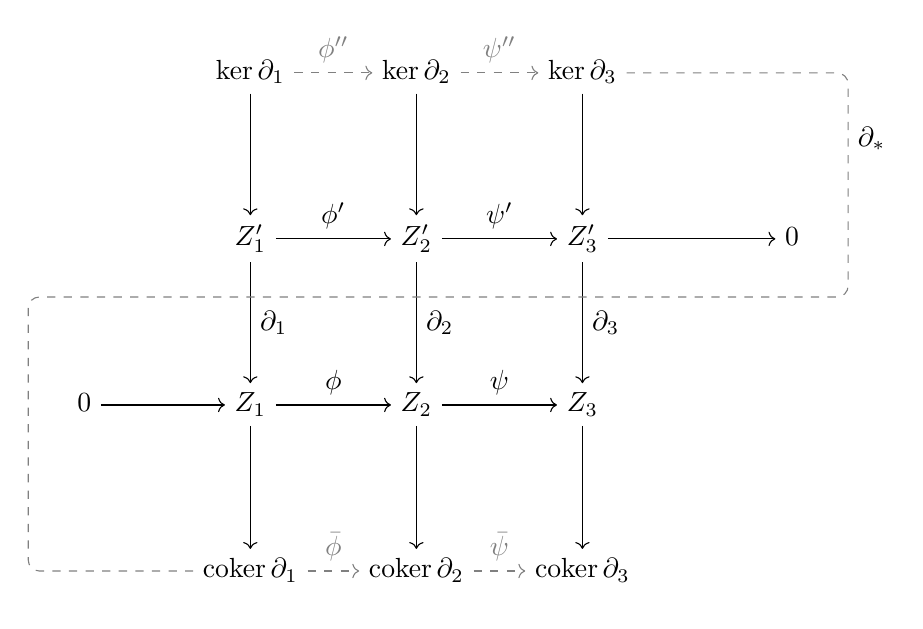
\begin{tikzpicture}
			\matrix[matrix of math nodes,column sep={60pt,between origins},row
			sep={60pt,between origins},nodes={asymmetrical rectangle}] (s)
			{
				&|[name=ka]| \ker \partial_1 &|[name=kb]| \ker \partial_2 &|[name=kc]| \ker \partial_3 \\
				%
				&|[name=A]| Z_1' &|[name=B]| Z_2' &|[name=C]| Z_3' &|[name=01]| 0 \\
				%
				|[name=02]| 0 &|[name=A']| Z_1 &|[name=B']| Z_2 &|[name=C']| Z_3 \\
				%
				&|[name=ca]| \coker \partial_1 &|[name=cb]| \coker \partial_2 &|[name=cc]| \coker \partial_3 \\
			};
			\draw [->]    (ka) edge (A)
			(kb) edge (B)
			(kc) edge (C)
			(A) edge node[auto] {\(\phi'\)} (B)
			(B) edge node[auto] {\(\psi'\)} (C)
			(C) edge (01)
			(A) edge node[auto] {\(\partial_1\)} (A')
			(B) edge node[auto] {\(\partial_2\)} (B')
			(C) edge node[auto] {\(\partial_3\)} (C')
			(02) edge (A')
			(A') edge node[auto] {\(\phi\)} (B')
			(B') edge node[auto] {\(\psi\)} (C')
			(A') edge (ca)
			(B') edge (cb)
			(C') edge (cc)
			;
			\draw[->,gray,dashed] (ka) edge node[auto] {\(\phi''\)}(kb)
			(kb) edge node[auto] {\(\psi''\)}(kc)
			(ca) edge node[auto] {\(\bar\phi\)} (cb)
			(cb) edge node[auto] {\(\bar\psi\)} (cc)
			;
			\draw[gray,dashed,rounded corners] (kc) -| node[auto,text=black,pos=.7]
			{\(\partial_*\)} ($(01.east)+(.5,0)$) |- ($(B)!.35!(B')$) -|
			($(02.west)+(-.5,0)$) |- (ca);
		\end{tikzpicture}\]
		donde $\coker\partial_i=Z_i/\partial_i$. (Este diagrama fue tomado de  \href{https://tex.stackexchange.com/questions/3892/how-do-you-draw-the-snake-arrow-for-the-connecting-homomorphism-in-the-snake-l}{\textbf{internet}}).
	\end{lema}
	\begin{obs}
		Intuitivamente, el $\coker$ nos da información de qué tan lejos está un homomorfismo de ser suprayectivo.
	\end{obs}
%\chapter{El teorema fundamental del álgebra homológica}
\section{Teorema fundamental del álgebra homológica}
	Primero introduciremos algo de notación
	\begin{defn}
		Diremos que una sucesión de complejos de cadena
		\[\begin{tikzcd}[column sep=small]
			&\cdots\arrow{r}&C_\bullet\arrow{r}{f}&D_\bullet\arrow{r}{g}&E_\bullet\arrow{r}&\cdots
		\end{tikzcd}\]
		es exacta en $D_\bullet$ si 
		\[\begin{tikzcd}[column sep=small]
			&\cdots\arrow{r}&C_p\arrow{r}{f_p}&D_p\arrow{r}{g_p}&E_p\arrow{r}&\cdots
		\end{tikzcd}\]
		es exacta para todo $p\in\Z$
	\end{defn}
	\begin{teo}[fundamental del álgebra homológica]
		Si 
		\[\begin{tikzcd}[column sep=small]
			&\cdots\arrow{r}&A_\bullet\arrow{r}{\phi}&B_\bullet\arrow{r}{\psi}&C_\bullet\arrow{r}&\cdots
		\end{tikzcd}\]
		es una sucesión exacta de complejos de cadena, entonces existen homomorfismos \[\delta_{*p}:H_p(C_\bullet)\to H_{p-1}(A_\bullet)\]
		tales que la sucesión
		\[\begin{tikzcd}[column sep=small]
			&\cdots\arrow{r}&H_p(A_\bullet)\arrow{r}{\bar\phi_p}&H_p(B_\bullet)\arrow{r}{\bar\psi_p}&H_p(C_\bullet)\arrow{r}{\delta_{*p}}&H_{p-1}(A_\bullet)\arrow{r}{\bar\phi_{p-1}}&H_{p-1}(B_\bullet)\arrow{r}&\cdots
		\end{tikzcd}\]
		es exacta.
	\end{teo}
	En el siguiente diagrama conmutativo se ve claramente qué está pasando:
	\[
	\begin{tikzcd}
		& & 0 \arrow{d} & 0 \arrow{d} & 0 \arrow{d} & \\
		& \cdots \arrow{r} & A_{p+1} \arrow{r}{\partial_{p+1}} \arrow{d}{i_{p+1}} & A_p \arrow{r}{\partial_p} \arrow{d}{i_p} & A_{p-1} \arrow{r} \arrow[d,magenta,"i_{p-1}"] & \cdots \\
		& \cdots \arrow{r} & B_{p+1} \arrow{r}{\partial_{p+1}} \arrow{d}{j_{p+1}} & B_p \arrow[r,magenta,"\partial_p"] \arrow[d,magenta,"j_p"] & B_{p-1} \arrow{r} \arrow{d}{j_{p-1}} & \cdots \\
		& \cdots \arrow{r} & C_{p+1} \arrow{r}{\partial_{p+1}} \arrow{d} & C_p \arrow{r}{\partial_p} \arrow{d} & C_{p-1} \arrow{r} \arrow{d} & \cdots \\
		& & 0 & 0 & 0 & \\
	\end{tikzcd}
	\]
	Explicamos un poco cómo definir el homomorfismo de conexión haciendo cacería de diagrama. Comenzamos con un ciclo $c\in C_p(A)$. Como $j_p$ es suprayectiva, existe un $a\in B_p$ tal que $j_p(a)=c$. Luego, $\partial_p(a)\in\ker j_{p-1}$, ya que, como el diagrama conmuta, $\partial_pj_p=j_{p-1}\partial_p$ y $c$ es un ciclo. Como la sucesión es exacta, $\ker j_{p-1}=\img i_{p-1}$, así que existe $a\in A_{p-1}$ tal que $i_{p-1}(a)=\partial_p(b)$. Este $a$ es un ciclo, ya que el diagrama conmuta, $i_{p-2}(a)=\partial(\partial(b))=0$, y la $i_{p-2}$ es inyectiva por exactitud, es decir, el único elemento al que va a dar el cero es el cero. Así que definimos $\delta_{*p}[c]=[a]$.
\section{Natrualidad del homomorfismo de conexión}
	\begin{teo}[Naturalidad del homomorfismo de conexión]
		\[\begin{tikzcd}[column sep=small]
			&0\arrow{r}&A_\bullet\arrow{r}{i}\arrow{d}{f}&B_\bullet\arrow{r}{j}\arrow{d}{g}&C_\bullet\arrow{r}\arrow{d}{h}&0\\
			&0\arrow{r}&A'_\bullet\arrow{r}&B'_\bullet\arrow{r}&C'_\bullet\arrow{r}&0
		\end{tikzcd}\]
		donde las filas son exactas.\par
		Entonces, el siguiente diagrama conmuta
		\[\begin{tikzcd}[column sep=small, row sep=large]
			& \cdots \arrow{r} & H_p(A) \arrow{r} \arrow{d}{\bar{f}} & H_p(B) \arrow{r} \arrow{d}{\bar{g}} & H_p(C) \arrow{r}{\delta_*} \arrow{d}{\bar{h}} & H_{p-1}(A) \arrow{r} \arrow{d}{\bar{f}} & H_{p-1}(B) \arrow{r} \arrow{d}{\bar{g}} & H_{p-1}(C) \arrow{r} \arrow{d}{\bar{h}} & \cdots \\
			& \cdots \arrow{r} & H_p(A') \arrow{r} & H_p(B') \arrow{r} & H_p(C') \arrow{r} & H_{p-1}(A') \arrow{r} & H_{p-1}(B') \arrow{r} & H_{p-1}(C') \arrow{r} & \cdots
		\end{tikzcd}\]
	\end{teo}
	Parece que ésta es una propiedad relacionada con la estructura de funtor de la homología.
\section{Lema de los cinco}
	\begin{lema}[de los cinco]
		Consideremos el diagrama conmutativo con filas exactas
		\[\begin{tikzcd}
			M_5\arrow{r}{f_5}\arrow{d}{h_5}&M_4\arrow{r}{f_4}\arrow{d}{h_4}&M_3\arrow{r}{f_3}\arrow{d}{h_3}&M_2\arrow{r}{f_2}\arrow{d}{h_2}&M_1\arrow{d}{h_1}\\
			N_5\arrow[r,swap,"g_5"]&N_4\arrow[r,swap,"g_4"]&N_3\arrow[r,swap,"g_3"]&N_2\arrow[r,swap,"g_2"]&N_1
		\end{tikzcd}\]
		Si $h_5,h_4,h_2$ y $h_1$ son isomorfismos, entonces $h_3$ también.
	\end{lema}
	¿En dónde se usará esto?

\chapter{Homología singular}
\section{Simplejos}
	Comenzaremos definiendo varios conceptos nuevos. Fijemos un entero $n\geq0$. Un \textbf{$n$-simplejo} es el convexo más pequeño en $\R^m$ ($m>n$) que contiene $n+1$ puntos $v_0,...,v_n$ que no viven en un hiperplano de dimensión menor que $n$.
	\begin{figure}[H]
		\centering
		\begin{subfigure}{0.23\textwidth}
			\centering
			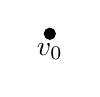
\begin{tikzpicture}[>=latex]
				% TikZ code for the 0-simplex
				\coordinate[label=below:$v_0$] (v0) at (0,0);
				\draw[fill=black] (v0) circle (2pt);
			\end{tikzpicture}
			\caption*{0-simplejo}
		\end{subfigure}
		\begin{subfigure}{0.23\textwidth}
			\centering
			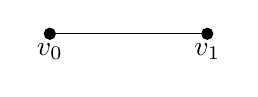
\begin{tikzpicture}[>=latex]
				% TikZ code for the 1-simplex
				\coordinate[label=below:$v_0$] (v0) at (0,0);
				\coordinate[label=below:$v_1$] (v1) at (2,0);
				\foreach \vertex in {v0,v1}
				\draw[fill=black] (\vertex) circle (2pt);
				\draw (v0) -- (v1);
			\end{tikzpicture}
			\caption*{1-simplejo}
		\end{subfigure}
		\begin{subfigure}{0.23\textwidth}
			\centering
			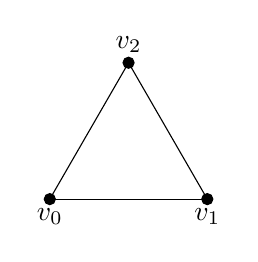
\begin{tikzpicture}[>=latex]
				% TikZ code for the 2-simplex
				\coordinate[label=below:$v_0$] (v0) at (0,0);
				\coordinate[label=below:$v_1$] (v1) at (2,0);
				\coordinate[label=above:$v_2$] (v2) at (1,{sqrt(3)});
				\foreach \vertex in {v0,v1,v2}
				\draw[fill=black] (\vertex) circle (2pt);
				\draw (v0) -- (v1);
				\draw (v1) -- (v2);
				\draw (v0) -- (v2);
			\end{tikzpicture}
			\caption*{2-simplejo}
		\end{subfigure}
		\begin{subfigure}{0.23\textwidth}
			\centering
			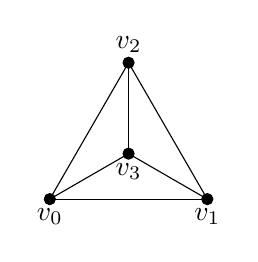
\begin{tikzpicture}[line join=bevel, scale=2]
				\coordinate[label=below:$v_0$] (v0) at (0,0);
				\coordinate[label=below:$v_1$] (v1) at (1,0);
				\coordinate[label=above:$v_2$] (v2) at (0.5,{sqrt(3)/2});
				\coordinate[label=below:$v_3$] (v3) at (0.5,{sqrt(3)/6});
				
				\draw (v1) -- (v2);
				\draw (v2) -- (v3);
				\draw (v0) -- (v1);
				\draw(v0) -- (v2);
				\draw (v0) -- (v3);
				\draw (v1) -- (v3);
				\draw (v2) -- (v3);
				
				% Vertices circles
				\foreach \vertex in {v0,v1,v2,v3}
				\draw[fill=black] (\vertex) circle (1pt);
			\end{tikzpicture}
			\caption*{3-simplejo}
		\end{subfigure}
	\end{figure}
		Lo denotaremos por $[v_0,…,v_n]$ y diremos que 	 $v_0,…,v_n$ son sus \textbf{vértices}. Y podemos escribirlo así: $[v_0,...,v_n]=\{t_0v_0+…+t_nv_n|t_i\geq0,t_0+…+t_n=1\}$.
		
		El \textbf{$n$-simplejo estándar} es $\Delta^n:=[e_1,…,e_n]$ donde $e_1,…,e_n$ es la base canónica de $\R^{n+1}$.
		
	\begin{figure}[H]
		\centering
		\begin{subfigure}{0.3\textwidth}
			\centering
			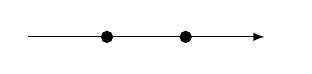
\begin{tikzpicture}[>=latex]
				% Axis
				\draw[->] (-1,0) -- (2,0) node[right]{};
				
				% Vertices
				\coordinate (v0) at (0,0);
				\coordinate (v1) at (1,0);
				
				% Edge
				\draw (v0) -- (v1);
				
				% Vertices circles
				\foreach \vertex in {v0,v1}
				\draw[fill=black] (\vertex) circle (2pt);
			\end{tikzpicture}
			\caption*{1-simplejo estándar}
		\end{subfigure}
		\begin{subfigure}{0.3\textwidth}
			\centering
			\begin{tikzpicture}[>=latex]
				% Axes
				\draw[->] (0,0) -- (2,0) node[right]{$x$};
				\draw[->] (0,0) -- (0,2) node[above]{$y$};
				
				% Vertices
				\coordinate (v0) at (1,0);
				\coordinate (v1) at (0,1);
				
				% Edges
				\draw (v0) -- (v1);
				
				% Vertices circles
				\foreach \vertex in {v0,v1}
				\draw[fill=black] (\vertex) circle (2pt);
			\end{tikzpicture}
			\caption*{2-simplejo estándar}
		\end{subfigure}
		\begin{subfigure}{0.3\textwidth}
			\centering
			\begin{tikzpicture}[>=latex]
				% Axes
				\draw[->] (0,0,0) -- (2,0,0) node[right]{$x$};
				\draw[->] (0,0,0) -- (0,2,0) node[above]{$z$};
				\draw[->] (0,0,0) -- (0,0,2) node[below left]{$y$};
				
				% Vertices
				\coordinate (v0) at (1,0,0);
				\coordinate (v1) at (0,1,0);
				\coordinate (v2) at (0,0,1);
				
				% Edges
				\draw (v0) -- (v1) -- (v2) -- cycle;
				
				% Vertices circles
				\foreach \vertex in {v0,v1,v2}
				\draw[fill=black] (\vertex) circle (2pt);
			\end{tikzpicture}
			\caption*{3-simplejo estándar}
		\end{subfigure}
	\end{figure}
	Y observemos que $\Delta^n=\{(t_0,…,t_n)\in\R^{n+1}|t_0+…+t_n=1\}$
	Para nosotros el orden de los vértices en $[v_0,…,v_n]$ es importante y siempre hay que tenerlo en mente.
	
	Dado un $n$-simplejo siempre tenemos la función:
	\begin{align*}
		(v_0,…,v_n):\Delta^n&\to[v_0,…,v_n]\\
		(t_0+…+t_n)&\mapsto t_0v_0+…+t_nv_n
	\end{align*}
	Y diremos que $(t_0,\cdots+t_n$ son las \textbf{coordenadas baricéntricas} del punto $t_0v_0+…+t_nv_n\in[v_0,…,v_n]$.
	
	Una \textbf{cara} de $[v_0,…,v_n]$ es el subsimplejo de generado por cualquier subconjunto no vacío de ${v_0,…,v_n}$. Cualquier cara 1-dimensional $[v_i,v_j]$ con $i<j$ vamos a considerarla orientada en orden ascendente:
	\vspace*{.7cm}
	
	\begin{center}
	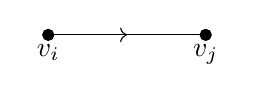
\begin{tikzpicture}
		%Vertices
		\coordinate[label=below:$v_i$] (vi) at (0,0);
		\coordinate[label=below:$v_j$] (vj) at (2,0);
		
		% Vertices circles
		\foreach \vertex in {vi,vj}
		\draw[fill=black] (\vertex) circle (2pt);
	
		% Edge
		\draw[postaction={decorate, decoration={markings, mark=at position 0.5 with {\arrow{>}}}}] (vi) -- (vj);
	\end{tikzpicture}
	\hspace{1cm}
	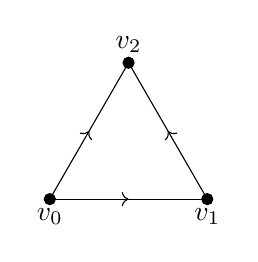
\begin{tikzpicture}
		% Vertices
		\coordinate[label=below:$v_0$] (v0) at (0,0);
		\coordinate[label=below:$v_1$] (v1) at (2,0);
		\coordinate[label=above:$v_2$] (v2) at (1,{sqrt(3)});
		
		% Vertices circles
		\foreach \vertex in {v0,v1,v2}
		\draw[fill=black] (\vertex) circle (2pt);
		
		% Edges
		\draw[postaction={decorate, decoration={markings, mark=at position 0.5 with {\arrow{>}}}}] (v0) -- (v1);
		\draw[postaction={decorate, decoration={markings, mark=at position 0.5 with {\arrow{>}}}}] (v1) -- (v2);
		\draw[postaction={decorate, decoration={markings, mark=at position 0.5 with {\arrow{>}}}}] (v0) -- (v2);
	\end{tikzpicture}
	\hspace{1cm}
	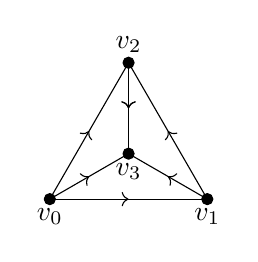
\begin{tikzpicture}[line join=bevel, scale=2]
		\coordinate[label=below:$v_0$] (v0) at (0,0);
		\coordinate[label=below:$v_1$] (v1) at (1,0);
		\coordinate[label=above:$v_2$] (v2) at (0.5,{sqrt(3)/2});
		\coordinate[label=below:$v_3$] (v3) at (0.5,{sqrt(3)/6});
		
	
		\draw[postaction={decorate, decoration={markings, mark=at position 0.5 with {\arrow{>}}}}] (v1) -- (v2);
		\draw[postaction={decorate, decoration={markings, mark=at position 0.5 with {\arrow{>}}}}] (v2) -- (v3);
		\draw[postaction={decorate, decoration={markings, mark=at position 0.5 with {\arrow{>}}}}] (v0) -- (v1);
		\draw[postaction={decorate, decoration={markings, mark=at position 0.5 with {\arrow{>}}}}] (v0) -- (v2);
		\draw[postaction={decorate, decoration={markings, mark=at position 0.5 with {\arrow{>}}}}] (v0) -- (v3);
		\draw[postaction={decorate, decoration={markings, mark=at position 0.5 with {\arrow{>}}}}] (v1) -- (v3);
		\draw[postaction={decorate, decoration={markings, mark=at position 0.5 with {\arrow{>}}}}] (v2) -- (v3);
		
		% Vertices circles
	\foreach \vertex in {v0,v1,v2,v3}
	\draw[fill=black] (\vertex) circle (1pt);
	\end{tikzpicture}
	\end{center}
	
	¿Cómo quedan orientadas las caras de dimensión 2?
	
\section{El complejo de cadenas singulares}
	Tomemos un espacio topológico  $X$  y un anillo asociativo con unidad $R$. Un \textbf{$n$-simplejo singular} es una función $\sigma:\Delta^n\to X$.
	
	El término ``singular" proviene de que no se le imponen condiciones a la función $\sigma$ salvo continuidad. Esto quiere decir que un simplejo singular puede verse bastante diferente de como lo imaginamos inicialmente.
	
	Definamos el siguiente conjunto 
	\[C_n(X):=\left\{\sum_{i=1}^mr_i\sigma_i|m\in\Z,r_i\in\R,\sigma_i\text{ es un simplejo singular}\right\}\]
	Que es el $R$-módulo libre generado por el conjunto de $n$-simplejos singulares. Los elementos de $C_n$ se llaman $n$-cadenas singulares. Queremos construir la siguiente sucesión:
	\begin{equation}\label{eq2.1}\begin{tikzcd}
		\cdots\arrow{r}&C_{n+1}(X)\arrow{r}{\partial_{n+1}}&C_n(X)\arrow{r}{\partial_n}&C_{n-1}(X)\arrow{r}{\partial{n-1}}&\cdots\arrow{r}{\partial_1}&C_0(X)
	\end{tikzcd}\end{equation}
	Para lo cual basta definir
	$\partial_n:C_n(X)\to C_{n-1}(X)$ como sigue: para un $n$-simplejo singular $\sigma:\Delta^n=[v_0,\ldots,v_n]\to X$,
	\[\partial_n(\sigma)=\sum_{i=0}^n(-1)^i\sigma|[v_0,\ldots,\hat{v}_i,\ldots,v_n]\]
	Donde $\sigma|[v_0,\ldots,\hat{v}_i,\ldots,v_n]$ es el siguiente $n-1$-simplejo singular: primero tomemos la $n-1$-cara de $\Delta^n$ que se obtiene al quitar el vértice $v_i$, es decir, $[v_0,\ldots,v_{i-1},v_{i+1},\ldots,v_n]$. Y luego simplemente componemos:
	$\partial_n:C_n(X)\to C_{n-1}(X)$ como sigue: para un $n$-simplejo singular $\partial_n:C_n(X)\to C_{n-1}(X)$ como sigue: para un $n$-simplejo singular $\sigma:\Delta^n=[v_0,\ldots,v_n]\to X$,
	\[\partial_n(\sigma)=\sum_{i=0}^n(-1)^i\sigma|[v_0,\ldots,\hat{v}_i,\ldots,v_n]\]
	Donde $\sigma|[v_0,\ldots,\hat{v}_i,\ldots,v_n]$ es el siguiente $n-1$-simplejo singular: primero tomemos la $n-1$-cara de $\Delta^n$ que se obtiene al quitar el vértice $v_i$, es decir, $[v_0,\ldots,\hat{v}_i,\ldots,v_n]:= [v_0,\ldots,v_{i-1},v_{i+1},\ldots,v_n]$. Y luego simplemente componemos:
	\[
	\begin{tikzcd}
		{[v_0,\ldots,v_n]} \arrow{r}{\sigma} & X \\
		{[v_0,\ldots,\hat{v}_i,\ldots,v_n]}\arrow[u,hook]&{[v_0,\ldots,v_{n-1}]}=\Delta^{n-1}\arrow{l}\arrow{u}[swap]{\sigma|[v_0,\ldots,\hat{v}_i,\ldots,v_n]}
		\arrow[from=1-1, to=2-2, phantom, "\circlearrowright"]
	\end{tikzcd}
	\]
	Donde la flecha de abajo es la función obvia: manda los vértices en orden y se brinca el $i$-ésimo. Y bueno, así queda definida la función $\partial_n$ en la base de $C_n$, y simplemente extendemos por linealidad a todo $C_n$. Ahora veamos una proposición:
	\begin{prop}
		$\partial_{n-1}\circ\partial_n=0$
	\end{prop}
	Con lo que la sucesión \eqref{eq2.1} es un complejo de cadenas que podemos llamar el \textbf{complejo de cadenas singulares de $X$}, que denotaremos por $C_\bullet(X)$. Y ahora podemos considerar sus grupos de homología y definir \[H_n(X;R):=H_n(C_\bullet(X))\] como el \textbf{$n$-ésimo grupo de homología singular de $X$ con coeficientes en $R$.}
\section{Primeras propiedades de la homología}
\subsection{La homología y las componentes arco-conexas}
\begin{prop}
	Sea $X=\bigsqcup X_i$ la descomposición en componentes arco-conexas del espacio topológico $X$, entonces
	\[H_n\left(\bigsqcup X_i,R\right)\cong \bigoplus H_n(X_i,R)\]
\end{prop}
\subsection{El 0-ésimo grupo de homología}
\begin{prop}
	Para cualquier espacio $X$, $H_0(X;R)$ es un suma directa de copias de $R$, una por cada componente arcoconexa.
\end{prop}
\subsection{La homología de un punto}
	 \begin{prop}
	 	Si $X$ consiste de un sólo punto, entonces
	 	\[H_n(X;R)=\begin{cases}R\qquad\text{si   } n=0\\
	 	0\qquad\text{si   } n\neq0
		 \end{cases}\]
	\end{prop}
	Para que esto no es totalmente intuitivo: nos gustaría que la homología de este espacio fuera 0 en todas las dimensiones. Vamos a componer esto en la siguiente sección.
\section{Homología reducida}\label{sec:6.4}
	La homología reducida es una variante de la homología singular que nos sirve para hacer cuentas en dimensiones bajas.
	
	\begin{defn}
		Sean $X$ un espacio topológico y $R$ un anillo asociativo con unidad. Los grupos de \textbf{homología reducida} de $X$ con coeficientes en $R$, que denotamos por $\tilde{H}(X;R)$, son los grupos de homología del siguiente complejo de cadenas:
	
		\[\begin{tikzcd}[column sep=small]
			\cdots \arrow[r] & C_p(X) \arrow[r, "\partial_p"] & C_{p-1}(X) \arrow[r, "\partial_{p-1}"] & C_{p-2}(X) \arrow[r] & \cdots \arrow[r] & C_1(X) \arrow[r, "\partial_1"] & C_0(X) \arrow[r, "\varepsilon"] & R \arrow[r] & 0
		\end{tikzcd}\]
		donde $\varepsilon(\sum n_i\sigma_i)=\sum n_i$ es el \textbf{mapeo de aumentación}.
	\end{defn}
	
	\begin{obs}
		Como el complejo de cadenas es idéntico al complejo de cadenas singulares salvo en los términos hasta la derecha, la homología reducida sólo podrá ser distinta de la homología singular en dimensión 0. Es decir,
		 $\tilde H_n(X;R)=H_n(X;R)$ para toda $n\geq 1$.
	\end{obs}
	
	\begin{ejer}[La homología reducida del espacio que es sólo un punto]
		Si $X=\{x\}$, entonces $\tilde H_0(X;R)=0$. 
	\end{ejer}
	\begin{proof}
		Recordemos cómo calculamos la 0-ésima hología singular de $X$. Como el último homomofismo en el complejo de cadenas singulares es $X\xrightarrow{\partial_0}0$, entonces el kernel es todo el grupo, así que $H_0(X)=C_0(X)/\img(\partial_1)$. Demostramos usando el mapeo de aumentación que este cociente es isomorfo a $R$. Luego,
		\[\begin{tikzcd}[column sep=small] 
			0\arrow[r]&\img\partial_1\arrow[r]&C_0(X)\arrow[r,"\varepsilon"]&R\arrow[r]&0
		\end{tikzcd}\]
		es una sucesión exacta corta. (Ver \hyperref[sucex]{prop} de sucesiones exactas).
				
		 Así que la sucesión del complejo de cadenas de la homología reducida es exacto en el nivel 0, es decir, $\ker(\varepsilon)=\img(\partial_1)=0$, de forma que $\tilde{H}_0(X;R)=0$
	\end{proof}
	\begin{ejer}
		En general, $H_0(X;R)=\tilde H_0(X;R)\oplus R$.
	\end{ejer}
	\begin{proof}
	 Por la definición de $\varepsilon$, sabemos que $\varepsilon|_{\img\partial_1}=0$. 
		
		Recordemos que en general, un mapeo que sale de un grupo pasa al cociente respecto a un subgrupo normal si su kernel está contenido en ese subgrupo. Esto quiere decir que tenemos un mapeo inducido $\bar{\varepsilon}:H_0(X;R)=C_0(X)/\img\partial_1\to R$. Este mapeo resulta ser suprayectivo, y además su kernel es $\ker\varepsilon/\img\partial_1=\tilde{H}_0$. En el lenguaje que hemos desarrollado, esto es tanto como decir que tenemos la sucesión exacta corta
		\[\begin{tikzcd}[column sep=small]
			0\arrow[r]&\tilde{H}_0(X;R)\arrow[r]&H_0(X;R)\arrow[r,"\bar\varepsilon"]&R\arrow[r]&0
		\end{tikzcd}\]
		Y a la mera hora $H_0(X;R)/\tilde{H}_0(X;R)\cong R$. De hecho, esto implica que $H_0(X;R)\cong\tilde{H}_0(X;R)\oplus R$. Para verlo, simplemente hay que notar que $\bar{\varepsilon}$ manda un elemento $g\in H_0(X;R)$ o bien al elemento 0, en cuyo caso está en $\tilde{H}_0(X;R)$, o bien a un elemento en $R$, que es el resto de su imagen. Estos dos grupos tienen intersección trivial y generan la suma directa $\tilde{H}_0(X;R)\oplus R$.
	\end{proof}

\section{Funtorialidad}
	En esta sección vamos a demostrar que, en el lenguaje categórico, la asociación que a cada espacio topológico le asigna su complejo de cadenas es funtorial. Y también, que la asignación que a cada espacio le asigna su $n$-ésimo grupo de homología es funtorial.
	
	Dicho de otra forma, lo que veremos es que funciones entre espacios topológicos inducen funciones entre los complejos de cadenas singulares y por lo tanto también funciones entre los grupos de homología singular, y además, composiciones van a composiciones y la identidad va a la identidad.
	
\section{Invarianza homotópica}
Primero \hyperref[def:func-homot]{recordemos} que 
\begin{defn}
	Dos funciones $f,g:X\to Y$ son \textbf{homotópicas} si existe una función $H:X\times I\to Y$ tal que
	\begin{align*}
		H(x,0)=f(x)\qquad\forall x\in X\\
		H(x,1)=g(x)\qquad\forall x\in X
	\end{align*}
	y se denota por $f\simeq g$.
\end{defn}
\begin{defn}
	Dos espacios $X$ y $Y$ son \textbf{homotópicamente equivalentes} si existen dos funciones llamadas \textbf{equivalencias homotópicas} $f:X\to Y$ y $g:Y\to X$ tales que $g\circ f\simeq Id_X$ y $f\circ g\simeq Id_Y$. Y se denota por $X\simeq Y$.
\end{defn}
Ahora sí:
\begin{teo}
	Si dos funciones $f,g:X\to Y$ son homotópicas, entonces inducen el mismo homomorfismo en el $n$-ésimo grupo de homología $f_*=g_*:H_n(X)\to H_n(Y)$ para toda $n$.
\end{teo}
\begin{coro}
	Si $f:X\to Y$ es una equivalencia homotópica, entonces la función inducida $f_*:H_n(X)\to H_n(Y)$ es un isomorfismo para toda $n$.
\end{coro}
\begin{proof}
	Usando el teorema y las propiedades de funtorialidad.
\end{proof}
\begin{ejem}
	Si $X\simeq \{x_0\}$, es decir $X$ es \textbf{contraible}, entonces \[H_n(X,R)=\begin{cases} R\qquad\text{si }n=0\\0\qquad\text{si }n\neq0\end{cases}\]
\end{ejem}
\section{Homología relativa}
\subsection{Construcción}

	La homología relativa es un tipo de homología singular que generaliza la homología reducida. El chiste será definir la homología del espacio ``ignorando lo que pasa dentro del subespacio".
	
	Tomemos $A\subseteq X$ espacios topológicos. Diremos que $(X,A)$ es una \textbf{pareja}. Notemos que $(C_\bullet(A))$ es un subcomplejo de $C_\bullet (X)$, así que podemos definir el complejo relativo
	\[
	C_\bullet(X,A)=C_\bullet(X)/C_\bullet(A)
	\]
	Y esto simplemente quiere decir que para toda $n$,
	\[
	C_n(X,A)=C_n(X)/C_n(A)
	\]
	de forma que las cadenas en $A$ se vuelven triviales.
	
	Es claro que el n-ésimo operador frontera restringido a $C_n(A)$ se mapea a $C_{n-1}(A)$, (pues la frontera de una cadena en $A$ no podría salirse de $A$). Esto quiere decir que el mapeo frontera está bien definido en el cociente. 
	\[\begin{tikzcd}[column sep=small]
		\cdots \arrow[r] & C_{n+1}(X,A) \arrow[r, "\partial_{n+1}"] & C_n(X,A) \arrow[r, "\partial_n"] & C_{n-1}(X,A) \arrow[r] & \cdots
	\end{tikzcd}\]
	Esto induce la homología dada por
	\[H_n(X,A)=\ker\partial_n/\text{img }\partial_{n-1}\]
		Ahora lo primero que pasa es que tenemos una sucesión exacta corta a la que aplicaremos el teorema fundamental del álgebra homológica:
		\[
		\begin{tikzcd}[column sep=small]
			0 \arrow[r] & C_\bullet(A) \arrow[r, hook, "i"] & C_\bullet(X) \arrow[r, two heads, "j"] & C_\bullet(X,A) \arrow[r] & 0
		\end{tikzcd}
		\]
		Así que obtenemos la \textbf{sucesión exacta larga de la pareja}
		\[\begin{tikzcd}[column sep=small]
			\cdots \arrow[r] & H_n(A) \arrow[r, "i_{*n}"] & H_n(X) \arrow[r, "j_{*n}"] & H_n(X,A) \arrow[r, "\delta_n"] & H_{n-1}(A) \arrow[r, "i_{*n-1}"] & H_{n-1}(X) \arrow[r, "i_{*p-1}"] & \cdots
		\end{tikzcd}\]
		\begin{obs}
			Si los grupos de homología de la pareja $C_p(X,A)$ fueran triviales, autimáticamente tedríamos que el mapeo inducido por la inclusión sería un isomorfismo. De hecho, esto es un si y sólo si. Así, los grupos de homología miden qué tan diferentes son los grupos de homología de $A$ y los de $X$.
		\end{obs}
		\begin{obs}
		Agregamos el comentario de que aunque el mapeo $\delta$ que usamos para completar la sucesión exacta larga de la pareja viene del teorema fundamental del álgebra homológica, y al recordar la demostración del teorema nos damos cuenta de que este mapeo actúa exactamente como el operador frontera original de $X$.
		\end{obs}
		\begin{obs}
			También es posible definir la \textbf{homología reducida de la pareja}. (Ver Hatcher). De hecho resulta que es igual a la homología de la pareja que acabamos de definir, es decir, $\tilde{H}_n(X,A)=H_n(X,A)$
		\end{obs}
		\begin{ejer}
			$H_n(X,\{x_0\})=H_n(X)$. 
		\begin{proof}[Solución]
			Usando la primera y la tercera de las observaciones anteriores, sabemos que existe la sucesión exacta larga de la pareja en homología reducida. Como $\tilde{H}_n(\{x_0\})\cong0$ para toda $n$, tenemos el isomorfismo deseado.
			
			\textcolor{red}{Esta prueba está en el Hatcher (p.118). En el \href{https://www.youtube.com/watch?v=CwVxrSoU_ZU}{video} este ejercicio aparece antes de definir la sucesión exacta larga de la pareja y sin el comentario sobre la homología reducia. ¿Será posible demostrarlo sin esas dos cosas?}
		\end{proof}
		\end{ejer}
\subsection{Funciones inducidas}
	\begin{obs}
		Una \hyperref[def:func-homot]{función entre parejas} $f:(X,A)\to(Y,B)$ induce una función $f_\#:C_\bullet(X,A)\to C_\bullet(Y,B)$ y por lo tanto también otra función $f_*H_n(X,A)\to H_n(Y,B)$.
	\end{obs}
	\begin{prop}
		Si dos funciones entre parejas $f,g:(X,A)\to(Y,B)$ son homotópicas por funciones entre parejas, entonces los mapeos inducidos $f_*$ y $g_*$ son iguales.
	\end{prop}
\subsection{Splitting lemma}\label{subsec:splitting}
Tomemos el caso en que hay una retracción $r:X\to A$, es decir, $ri=id_A$ donde $i$ es la inclusión. Esto implica que $(ri)_*=r_*i_*=id_{H_n(A)}$, así que $r_*i_*$ es inyectiva, y de hecho podemos partir la sucesión exacta de la pareja en sucesiones exactas cortas de la forma
\[\begin{tikzcd}[column sep=small]
	0\arrow[r]&H_n(A)\arrow[r,"i_*"]&H_n(X)\arrow[r,"j_*"]&H_n(X,A)\arrow[r]&0
\end{tikzcd}\]
Pero hay más:
\begin{lema}[Splitting lemma]
	Para cualquier sucesión exacta corta de grupos abelianos
	\begin{tikzcd}[column sep=small]
		0\arrow[r]&A\arrow[r,"i"]&B\arrow[r,"j"]&C\arrow[r]&0
	\end{tikzcd}
	lo siguientes enunciados son equivalentes:
	\begin{enumerate}
		\item [(a)] Hay un homomorfismo $p:B\to A$ tal que $pi=id_A$.
		\item[(b)] Hay un homomorfismo $q:C\to B$ tal que $qj=id_C$.
		\item[(c)] Hay un isomorfismo $B\approx A\oplus B$ que hace conmutar el siguiente diagrama:
		\[\begin{tikzcd}[column sep=small,row sep=small]
			&&B\arrow[rd,"j"]\arrow[dd,"\approx"]\\
			0\arrow[r]&A\arrow[ru,"i"]\arrow[rd]&&C\arrow[r]&C\\
			&&A\oplus C\arrow[ru]
		\end{tikzcd}\]
		con los mapeos obvios en el último renglón, $a\mapsto(a,0)$ y $(a,c)\mapsto c$.
	\end{enumerate}
	En este caso decimos que la sucesión se \textbf{separa} (splits).
\end{lema}
\begin{obs}\leavevmode
	\begin{itemize}
	\item $C$ es libre (incluso si no es abeliano) si y sólo si la sucesión se separa.
	\item Una retracción $r:X\to A$ hace que $H_n(X)\approx H_n(A)\oplus H_n(X,A)$.
	\end{itemize}
\end{obs}
\subsection{La sucesión exacta de la tercia}
	Si $Z\subseteq Y\subseteq X$ son espacios topológicos, es inmediato por definición que
	\[C_\bullet(Z)\leq C_\bullet(Y\leq C_\bullet(X))\]
	Y al tomar el cociente por $Z$, obtenemos 
	\[\begin{tikzcd}[column sep=small]
		C_\bullet(Y,Z)\arrow[r,hook]&C_\bullet(X,Z)\arrow[r]&\frac{C_\bullet(X,Z)}{C_\bullet(Y,Z)}=C_\bullet(X,Y)
	\end{tikzcd}\]
	Usando un teorema de isomorfismo en la última igualdad para ver que $\frac{C_\bullet(X)/C_\bullet(Z)}{C_\bullet(Y)/C\bullet(Z)}=C\bullet(X,Y)$. Aplicamos el teorema fundamental del álgebra homológica y obtenemos la \textbf{sucesión exacta de la tercia}
	\[\begin{tikzcd}[column sep=small]
		\cdots\arrow[r]&H_n(Y,Z)\arrow[r,"i_*"]&H_n(X,Z)\arrow[r,"j_*"]&H_n(X,Y)\arrow[r,"\delta"]&H_{n-1}(Y,Z)\arrow[r,"i_*"]&\cdots
	\end{tikzcd}\]
\section{Escisión}\label{sec:escisión}
Este resultado hace mucho más precisa la noción de que la homología de la pareja es la homología del espacio ``ignorando lo que pasa en el subespacio".

Sean $Z\subseteq A\subseteq X$ tales que la cerradura de $Z$ está contenida en el interior de $A$. Entonces
\[(X-Z,A-Z)\hookrightarrow (X,A)\]
induce un isomorfismo
\[H_n(X-Z,A-Z)\to H_n(X,A)\qquad\forall n\]
Equivalentemente, para subespacios $A,B\subseteq X$ cuyos interiores cubren a $X$, la inclusión
\[(B,A\cap B)\hookrightarrow (X,A)\]
induce un isomorfismo
\[H_n(B,A\cap B)\to H_n(X,A)\qquad\forall n\]

\section{La homología de un cociente}
	Dados un espacio topológico $X$ y un subespacio $A\subseteq X$, podemos considerar el espacio $X/A$, que consiste en identificar todos los puntos de $A$. Este espacio es como $X$ pero `ìgnordando todo lo que pasa en $A$. Esto nos recuerda a la homología de la pareja, y surge naturalmente la pregunta: ¿hay alguna relación entre $H_n(X,A)$ y $H_n(X/A)$? Necesitamos ciertas condiciones:
	
	\begin{defn} Decimos que $(X,A)$ es una \textbf{buena pareja} si $A$ es cerrado y es retracto fuerte por deformación de alguna vecindad en $X$.
	\end{defn}
	
	El arete hawaiiano con el punto de pegado no es un buen par porque cualquier vecindad de dicho punto contiene un círculo entero, así que no se puede retraer por deformación.
	
	\begin{teo}Sea $(X,A)$ un buen par, entonces
		\[q:(X,A)\to(X/A,A/A)\]
		induce isomorfismos para toda $n$ de la forma
		\[q_{*}:H_n(X,A)\to H_n(X/A,A/A)\cong \tilde{H}_n(X/A)\]
		donde la tilde denota la homología reducida.
	\end{teo}
	
	En la demostración se usa lema de los 5, invarianza homotópica, etc.
	
	\begin{coro}
		Sea $(X,A)$ un buen par. Entonces tenemos la siguiente sucesión exacta larga:
		\[\begin{tikzcd}[column sep=small]
			\cdots \arrow[r] & \tilde{H}_n(A) \arrow[r] & \tilde{H}_n(X) \arrow[r] & \tilde{H}_n(X/A) \arrow[r] & \tilde{H}_{n-1}(A) \arrow[r] & \tilde{H}_{n-1}(X) \arrow[r] & \tilde{H}_{n-1}(X/A) \arrow[r] & \cdots
		\end{tikzcd}\]
	\end{coro}
	
\section{Homología de la esfera y aplicaciones}
	\begin{teo}[Homología de la esfera]
		\[\tilde H_i(S^n;R)=\begin{cases}R\qquad\text{si   } n=i\\
			0\qquad\text{si   } n\neq i
		\end{cases}\]
	\end{teo}
	\begin{teo}[del punto fijo de Bruwer]
		Sean $n\geq2$ y  $f:D^n\to D^n$, entonces $f$ tiene un punto fijo.
	\end{teo}
	\begin{teo}[Homología de la cuña]
		Consideremos una cuña de espacios $\bigvee_{\alpha\in I}X_\alpha$ tal que $(X_\alpha,x_\alpha)$ es una buena pareja para toda $\alpha$, donde $x_\alpha$ es el punto de pegado. Entonces, las inclusiones $i_\alpha:X_\alpha\hookrightarrow\bigvee_{\alpha\in I}$ inducen un isomorfismo
		\[\bigoplus i_{\alpha*}:\bigoplus_{\alpha\in I}\tilde{H}_n(X_\alpha)\to\tilde{H}_n\left(\bigvee_{\alpha\in I}\right)\]
	\end{teo}
	\begin{teo}[Invarianza de la dimensión]
		Sean $U\subseteq\R^n$ y $V\subseteq\R^m$ abiertos. Si $U$ y $V$ son homeomorfos, entonces $n=m$.
	\end{teo}

\section{La sucesión de Mayer-Vietoris}
	Sea $X$ un espacio topológico y $A,B\subseteq X$ tales que $X=\Int A\cup \Int B$. Entonces tenemos la siguiente sucesión exacta larga en homología reducida:
	\[\begin{tikzcd}[column sep= small]
		\cdots \arrow[r] & H_n(A\cap B) \arrow[r,"\Phi"] & H_n(A) \oplus H_n(B) \arrow[r,"\Psi"] & H_n(X) \arrow[r,"\delta"] & H_{n-1}(A\cap B) \arrow[r] &\cdots
	\end{tikzcd}\]
	Para entender de dónde salió esta sucesión, debemos fijarnos en los subgrupos de cadenas $C_n(A+B)$ formado por sumas de cadenas en $A$ y cadenas $B$. Es posible construir un complejo de cadenas, ya que el homomorfismo frontera de todo el espacio, $\partial:C_n(X)\to C_{n-1}(X)$ se restringe correctamente a $C_n(A+B)\to C_{n-1}(A+B)$. Usando la maquinaria del \hyperref[sec:escisión]{teorema de escisión}, se demuestra que la inclusión $C_n(A+B)\hookrightarrow C_n(X)$ induce isomorfismos en la homología. Luego, tenemos para toda $n$ la sucesión exacta corta:
	\[\begin{tikzcd}[column sep=small]
		0\arrow[r]&C_n(A\cap B)\arrow[r,"\varphi"]&C_n(A)\oplus C_n(B)\arrow[r,"\psi"]&C_n(A+B)\arrow[r]&0
	\end{tikzcd}\]
	donde $\varphi(x)=(x,-x)$ y $\psi(x,y)=x+y$. Esta forma de definir las funciones nos asegura que la sucesión sea exacta, como sigue. Es fácil ver que $\psi\varphi=0$, por lo que $\img\varphi\subseteq\ker\psi$. También $\ker\psi\subseteq\img\varphi$, ya que si $(x,y)\overset{\psi}{\mapsto}(0,0)$, entonces $x=-y$, así que tanto $x$ como $y$ están en $A$ y en $B$, es decir, $(x,y)\in\C_n(A\cap B)$; y  claramente está en la imagen de $\varphi$. También es fácil ver que $\ker\varphi=0$, y que $\img\psi=C_n(A+B)$.
	
	Aplicando el teorema fundamental del álgebra en la sucesión exacta corta de complejos de cadenas inducidos por estas sucesiones exactas cortas en cada $n$, se obtiene la sucesión de Mayer-Vietoris.
	
	Es posible decir cómo actúa el mapeo de aumentación. Por lo que dijimos sobre el teorema de escisión, un elemento en $[w]\in H_n(X)\cong H_n(A+B)$ es de la forma $[a+b]$ para cadenas $a\in C_n(A)$ y $b\in C_n(B)$ cuya suma $a+b$ es un ciclo, es decir, $\partial(a+b)=0$. Luego, $\partial(a)=-\partial(b)$ es un ciclo en $H_{n-1}(A\cap B)$, así que es el representante perfecto para la clase de equivalencia a la que vamos a mandar a $[w]$.
	
	Todo lo dicho hasta ahora se resume a continuación
	\begin{equation*}
	\begin{aligned}
	\begin{array}{c@{\hspace{2cm}}c}
			i:A\cap B\hookrightarrow A\\
			j:A\cap B\hookrightarrow B &\Phi(x)=(i_*x,-j_*x)\\
			k:A\hookrightarrow X&\Psi(y,z)=k_*y+\ell_*z\\
			\ell:B\hookrightarrow X
	\end{array}\\ \\
	[w]=[a+b]\overset{\delta}{\mapsto}[\partial(a)]=[-\partial(b)]\qquad\text{para ciertas }a\in C_n(A),b\in C_n(B)
	\end{aligned}
	\end{equation*}

	\begin{ejem}
		\href{https://math.stackexchange.com/questions/58311/the-homology-groups-of-t2-by-mayer-vietoris}{Es posible} calcular la homología del toro usando la sucesión de Mayer-Vietoris, aunque no basta con escribir la sucesión exacta: hay que entender cómo actúan los homomorfismos.
	\end{ejem}
	\begin{obs}
		Se puede dar una versión de esta sucesión para $X=A\cup B$ tales que $A$ y $B$ son retractos por deformación de ciertas vecindades $U$ y $V$ donde $U\cap V$ es retracto de $A\cap B$.
		
		En particualar, si $X$ es un \hyperref[chap:CCW]{complejo CW} y $A,B\subseteq X$ son subcomplejos CW, entonces es posible demostrar que existen tales vecindades, y obtenemos la misma sucesión de Mayer-Vietoris,
		\[\begin{tikzcd}[column sep= small]
			\cdots \arrow[r] & \tilde{H}_n(A\cap B) \arrow[r] & \tilde{H}_n(A) \oplus \tilde{H}_n(B) \arrow[r] & \tilde{H}_n(X) \arrow[r] & \tilde{H}_{n-1}(A\cap B) \arrow[r] &\cdots
		\end{tikzcd}\]
		Sólo que ahora $A$ y $B$ no tienen que ser abiertos y no tiene que ser cierto que $\Int A\cup\Int B=X$.
	\end{obs}
\begin{ejem}\label{ejem:toroCWMV}
	\textcolor{red}{En mis notas de clase hay un modo de calcular $H_1$ y $H_0$ del toro visto como complejo CW con subcomplejos:}
	
	Cuando vemos el toro $S^1\times S^1$ como el cociente de un cuadrado con los lados identificados, tenemos una estructura de complejo CW con una 0-celda, dos 1-celdas y una 2-celda. Aquí, podemos tomar $A=D^2$ y $B=S^1\vee S^1$.
	
	Casi todos los grupos de homología se hacen cero \textcolor{red}{(no veo por qué)} (aquí hay que usar que la homología de la cuña es la suma de las homologías de los "cuñandos"), y que la homología de $S^1$ es cero cuando el subíndice es mayor o igual que 2.
	
	En fin, para $m>2$, $\tilde H_m(X)=0$. Y es fácil ver que $H_1(S^1\times S^1)\cong R\oplus R$. Pero para $H_2(S^1\times S^1)$ algo falta…
	
\end{ejem}

\section{Representantes de la homología de la esfera}
	En esta sección usaremos $R=\mathbb Z$. 
	
	Nuestro método será encontrar generadores para la homología relativa $H_n(D^n,\partial D^n)$ ya que ésta debe ser isomorfa a $H_n(S^n)$. Y lo primero que vamos a hacer va a ser reemplazar esa pareja por la siguiente, a la que también es isomorfa: $(\Delta^n,\partial\Delta^n)$.
\begin{prop}
	 La función identidad $Id:\Delta^n\to\Delta^n$ es un ciclo que genera $H_n(\Delta^n,\partial\Delta^n)\cong\Z$.
	 \begin{proof}
	 	Primero notemos que la identidad sí es un ciclo en el grupo de homología relativa, ya que el kernel mapeo frontera $C_n(\Delta^n)\xrightarrow{\partial_n}C_{n-1}(\Delta^n)$ justamente está metido en el subgrupo $C_n(\partial\Delta^n)\leq C_n(\Delta^n)$. (Un homomorfismo de grupos pasa al cociente si el kernel está metido en el subgrupo normal).
	 	
	 	Ahora sí, hacemos inducción en $n$. (...)
	 	
%	 	Si $n=0$, entonces $\Delta^0=\{e_0\}$ es un punto y su frontera es el vacío. Luego $H_0(\Delta^0,\partial\Delta^0)=H_0(\Delta^0)=\mathbb Z=\langle[e_0]\rangle$.
%	 	
%	 	Ahora supongamos para $n$ y demostremos para $n+1$. Definamos $\Lambda$ como la unión de todas las $n-1$ caras en la frontera salvo alguna. Luego
%	 	$$
%	 	H_n(\Delta^n,\partial\Delta^n)\to^\delta H_n(\partial\Delta^n,\Lambda)\leftarrow^{\iota}H_{n-1}(\Delta^{n-1},\partial\Delta^{n-1})
%	 	$$
%	 	Luego como puedo retraer el simplejo en el $\Lambda$,
%	 	$$
%	 	H_{n-1}(\Delta^{n-1},\partial\Delta^{n-1})=0
%	 	$$
%	 	Así que (creo que) incluyendo el de en medio la primera ecuación en este anterior, obtenemos que $\delta$ es un isomorfismo.
%	 	
%	 	Para checar $\iota$, 
%	 	$$
%	 	H_{n-1}(\Delta^{n},\Lambda)\cong H_{n-1}(\partial\Delta^n/\Lambda)\\
%	 	H_{n-1}(\Delta^{n-1},\partial\Delta^{n-1})\cong H_{n-1}(\partial\Delta^{n-1}/\partial\Delta^{n-1})
%	 	$$
%	 	Y los dos de la derecha deben ser isomorfos. Hay un cuadrado conmutativo abajo de la inclusión $\iota$. Luego $\iota_{n-1}$ genera por hipótesis inductiva…
	 \end{proof}
\end{prop}
	Ahoara pensemos que $S^n$ es la unión de dos simplejos estándar pegados por su frontera, que denotaremos por $\Delta_1^n\cup_{\partial\Delta^n}\Delta_2^n$.
\begin{prop}
	$\Delta^n_1-\Delta^n_2$ es un generador de $H_n(S^n)$ para $n>0$.
\end{prop}
\section{Grado de una función entre esferas}
	Consideremos $f:S^n\to S^n$, que induce una función $f_*:\tilde H_n(S^n)\cong \mathbb Z\to \tilde H_n(S^n)\cong\mathbb Z$ de manera que $f_*$ no tiene de otra que ser de la forma $f_*(n\alpha)=dn\alpha$.
	\begin{defn}
		En la notación de arriba, el \textbf{grado} de $f$ es $d$.
	\end{defn}
	\begin{prop}\leavevmode
		
		\begin{enumerate}
			\item $\text{deg }Id=1$. Por funtorialidad.
			\item Si $f$ no es suprayectiva, entonces $\text{deg }(f)=0$. Como $f$ no es suprayectiva podemos escoger un punto $x\notin\text{img }f$. Tenemos los siguientes diagramas:
				\begin{figure}[H]
					\centering
					\begin{subfigure}[b]{0.4\textwidth}
						\centering
						\begin{tikzcd}[column sep=small]
							& S^2 - x \arrow[rd,hook] \\
							& S^2 \arrow[u, "f"] \arrow[r, "f"] & S^2
						\end{tikzcd}
					\end{subfigure}
					\qquad\qquad
					\begin{subfigure}[b]{0.4\textwidth}
						\centering
						\begin{tikzcd}[column sep=small]
							& \tilde{H}_n(S^2 - x) \cong 0 \arrow[rd,hook] \\
							& \tilde{H}_n(S^2) \arrow[u, "f_*"] \arrow[r, "f_*"] & \tilde{H}_n(S^2)
						\end{tikzcd}
					\end{subfigure}
				\end{figure}
				Y como el primero es conmutativo, el segundo también, y entonces $f_*$ es constante.
			\item $f\simeq g$ entonces $\deg f=\deg g$. Por invarianza homotópica las funciones inducidas son iguales.
			\item $\deg(fg)=\deg(f)\deg(g)$
			\item Si $f$ es una reflexión que intercambia los hemisferios, entonces $\deg(f)=-1$.
			
			Esto se debe a que, como vimos en la sección anterior, la $n$-esfera vista como la unión de dos simplejos estándar, $S^n=\Delta_1^n\cup_{\partial\Delta^n}\Delta_2^n$, tiene como generador del $n$-ésimo grupo de homología a la cadena $\Delta_1^n-\Delta_2^n$. La reflexión que intercambia estos simplejos justamente envía el generador a su negativo.
			\item La función antipodal $-Id:S^n\to S^n$ tiene grado $(-1)^{n+1}$. Es decir,
			\[\deg (-Id)=\begin{cases}1\qquad\text{ si }n\text{ es impar}\\
				-1\qquad\text{ si }n\text{ es par}\end{cases}\]
			\item Si $f$ no tiene puntos fijos, entonces $\deg (f)=(-1)^{n+1}$. Más aún, si $f$ no tiene puntos fijos, es homotópica al mapeo identidad.
			
			Si $x\neq f(x)$, el segmento de línea en $\R^{n+1}$ que pasa por $f(x)$ y $-x$, dado por $(1-tf(x))-tx$, no pasa por el origen. Esto nos permite definir una homotopía $(1-tf(x))-tx/|(1-tf(x))-tx|$ entre $f$ y el mapeo antipodal. 
		\end{enumerate}
	\end{prop}
\subsection{Grado local}\label{subsec:grloc}
	Siguiendo a Hatcher,
	\begin{defn}
		Supongamos que $f:S^n\to S^n$ es tal que la imagen inversa de algún $y\in S^n$ consiste de una cantidad finita de puntos, digamos $f^{-1}(y)=\{x_1,...,x_m\}$. Tomemos una familia de abiertos disjuntos $U_1,...,U_m$ que contengan a cada $x_i$, y que vayan a dar a una vecindad $V$ de $y$ bajo $f$. Mediante un diagrama conmutativo, usando escisión y la sucesión exacta larga, Hatcher argumenta que el homomorfismo $f_*$ originalmente definido así:
		\[H_n(S^n,S^n-x_i)\xleftarrow{\cong}H_n(U_i,U_i-x_i)\xrightarrow{f_*}H_n(V,V-y)\]
		es de la forma $f_*:\Z \to \Z$, la multiplicación por un número que se llama el **grado local** de $f$ y se denota $\deg f|x_i$.
	\end{defn}
	Supongamos que $f:S^n\to S^n$ es tal que la imagen inversa de algún $y\in S^n$ consiste de una cantidad finita de puntos, digamos $f^{-1}(y)=\{x_1,...,x_m\}$. Tomemos una familia de abiertos disjuntos $U_1,...,U_m$ que contengan a cada $x_i$, y que vayan a dar a una vecindad $V$ de $y$ bajo $f$. Mediante un diagrama conmutativo, usando escisión y la sucesión exacta larga, Hatcher argumenta que el homomorfismo $f_*$ originalmente definido así:
	\[H_n(S^n,S^n-x_i)\xleftarrow{\cong}H_n(U_i,U_i-x_i)\xrightarrow{f_*}H_n(V,V-y)\]
	es de la forma $f_*:\Z \to \Z$, la multiplicación por un número que se llama el **grado local** de $f$ y se denota $\deg f|x_i$.
	
	Y luego:
	\begin{teo}
		$\deg f=\sum_i\deg f|_{x_i}$
	\end{teo}
	Agregamos otra proposición:
	\begin{prop}
		El grado de la \hyperref[fsusp]{suspensión} $Sf:S^{n+1}\to S^{n+1}$ de una función $f:S^n\to S^n$ es igual al grado de $f$.
	\end{prop}
\subsection{Teorema de la bola peluda}
	\begin{teo}[de la bola peluda]
		$S^n$ tiene un campo vectorial que no se anula en ningún punto si y sólo si $n$ es impar.
	\end{teo}

\subsection{Acciones libres en la esfera}
	\begin{teo}[Acciones libres en la esfera]
		$\Z/2\Z$ es el único grupo no trivial que \hyperref[sec:acciones]{actúa} libremente en $S^n$ si $n$ es par.
	\end{teo}

\chapter{Complejos CW}\label{chap:CCW}
\section{Construcción y propiedades básicas}
	Establezcamos algo de notación
	\begin{itemize}
		\item $D^n=\{x\in\mathbb R^n:|x|\leq1\}$ es el $n$-disco cerrado.
		\item $S^n=\{x\in\mathbb R^n:|x|=1\}$ es la $n$-esfera.
		\item $e^n=\{x\in\mathbb R^n:|x|<1\}$ es la $n$-célula abierta o sólo la $n$-célula.
	\end{itemize}
	De tal forma que
	\begin{itemize}
		\item $\partial D^n=S^{n-1}$
		\item $D^n=e^n\cup S^{n-1}$ como conjuntos (no se usa la topología de la unión disjunta)
		\item Y bueno debe ser cierto que $e^0=\{pt\}$.
	\end{itemize}
	\begin{defn}
		Un espacio $X$ es un complejo $CW$ si se puede construir mediante el siguiente procedimiento:
		\begin{enumerate}
			\item Comenzamos con un espacio discreto $X^0$ que se llama el 0-esqueleto.
			\item El $n$-esqueleto $X^n$ lo obtengo a partir del $n-1$-esqueleto $X^{n-1}$ pegando $n$-células $e^n_\alpha$ vía funciones $\varphi_\alpha:S^{n-1}\to X^{n-1}$. Formalmente tenemos el espacio
			\[X^n=X^{n-1}\bigsqcup_\alpha D_\alpha^n\Big/\sim\qquad\qquad x\sim\varphi_\alpha(x)\quad\text{ si }\quad x\in\partial D^n_\alpha\]
			\textit{Se trata de tomar puntos y unirlos con líneas, y luego tomar líneas y rellenar con discos, etc...}
			\item Podríamos terminar en una cantidad finita de pasos, digamos $m$, y obtenemos que $X=X^m$, pero también puedo continuar pegando células de dimensión arbitrariamente grande y obtenemos $X=\bigcup_n X^n$. En este caso $X$ tiene la topología débil: $A\subseteq X^n$ es abierto (cerrado) $\iff A\cap X^n$ es abierto (cerrado) $\forall n$.
		\end{enumerate}
	\end{defn}
	\begin{defn}
		Si $X=X^n$ para algún $n\in\mathbb N$, decimos que $X$ es de dimensión finita y definimos la dimensión de $X$ como la dimensión de la célula más grande que adjunté. Formalmente, $\dim X=\min \{n:X^n=X\}$.
	\end{defn}
	\begin{ejem}\leavevmode
		\begin{itemize}
			\item Los 0-complejos CW son gráficas.
			\item $S^n$ es un complejo CW.
			\item El espacio proyectivo real. Inicialmente definido como $\R P^n=\R^{n+1}-\{0\}/x\sim\lambda x$ para $\lambda\neq0$, podemos tomar representantes de las líneas en la esfera para obtener que $\R P^n=S^n/x\sim -x$. 
			
			Esto es equivalente a tomar cualquiera de los hemisferios de la esfera, $D^{n}$, e identificar los puntos de su frontera con el mapeo antipodal. A su vez, esto es equivalente a tomar la esfera de dimensión $n-1$, que es la frontera del disco, identificar antipodalmente, y agregar el interior del $n$-disco. ¡Y la $n-1$ esfera con esa identificación es justamente $\R P^{n-1}$!
			
			En resumen, y haciendo inducción:
				\begin{align*}
					\R P^n&=\R^{n+1}-\{0\}/x\sim\lambda x,\qquad\lambda\neq0\\
					&=S^n/x\sim-x\\
					&=D^n/x\sim-x,\qquad x\in\partial D^n=S^{n-1}\\
					%&=\left(S^{n-1}/x\sim-x\right)\cup e^n\\
					&=\R P^{n-1}\cup e^n\\
					&=\R P^{n-2}\cup e^{n-1}\cup e^n\\
					&=e^0\cup e^1\cup\ldots\cup e^n
				\end{align*}
				donde las funciones de pegado son justamente las antipodales.
			\item El espacio proyectivo complejo. Como en el caso real, el espacio proyectivo complejo, inicialmente definido como $\C^{n+1}-\{0\}/x\sim\lambda x$ para $\lambda\neq0$, se puede definir únicamente en la esfera $S^{2n+1}$. Igualito que en el caso real, es posible tomar un disco $D^{2n}$ e identificar los puntos antípodas en su frontera. Por ahora no especificaremos cómo, pero resulta que:
			\[\C P^n=e^0\cup e^2\cup\ldots e^{2n}\]
		\end{itemize}
	\end{ejem}
	\begin{ejer}
		Todo complejo $CW$ es semilocalmente simplemente conexo. Es decir, todo complejo $CW$ tiene cubriente universal.
	\end{ejer}
	\begin{defn}
		Para cada $n$-celda de un complejo CW $e^n_\alpha$, tenemos la \textbf{función característica}, que es de la forma $\Phi_\alpha:D^n_\alpha\to X^n$ y está definida como una composición de acuerdo al siguiente diagrama:
%		\[\begin{tikzcd}
%			&e^n_\alpha \ar[rd] \ar[d, hook] & X^{n-1} \sqcup D_\alpha^n \ar[d, "\text{proyección al cociente}"] \\
%			&D^n_\alpha \ar[ur,hook] \ar[r, "\Phi_\alpha"'] & X^n
%		\end{tikzcd}\]
	\[
	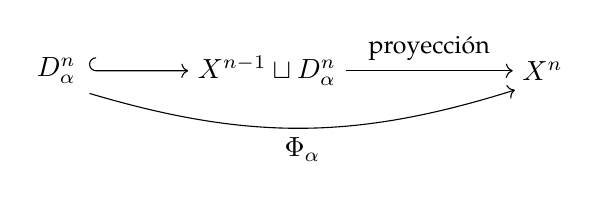
\begin{tikzpicture}
		% Nodes
%		\node (EA) at (-2,0) {$e^n_\alpha$};
		\node (A) at (0,0) {$D^n_\alpha\quad$};
		\node (B) at (2.5,0) {$X^{n-1}\sqcup D^n_\alpha$};
		\node (C) at (6,0) {$X^n$};
		
		% Arrows
%		\draw[->] ([xshift=2ex,yshift=1ex] EA) arc (90:270:0.5ex)--(A);
		\draw[->] ([xshift=2ex,yshift=1ex] A) arc (90:270:0.5ex)--(B);
		\draw[->] (B) -- node[above] {\small{proyección}} (C);
		
		% Curved arrow below
		\draw[->, bend right=17] ([xshift=7pt]A.south) to node[below] {$\Phi_\alpha$} ([xshift=-10pt]C.south);
	\end{tikzpicture}
	\]
	que extiende a la función de pegado $\varphi_\alpha$ y es un homeomorfismo del interior de $D_\alpha^n$ en $e^n_\alpha$.
	\end{defn}
	\begin{defn}
		Sea $X$ un complejo $CW$. Un \textbf{subcomplejo CW} $Z$ es un subespacio cerrado que además es unión de células de $X$.	
	\end{defn}
	\begin{obs}
		Para un subcomplejo $Z$,
		\begin{itemize}
			\item $Z\subseteq X$ es una buena pareja ($Z$ es retracto por deformación de una vecindad de $X$)
			\item $X/Z$ (el espacio que obtiene al colapsar $Z$ a un punto) es un complejo $CW$.
		\end{itemize}
	\end{obs}
	\begin{obs}[Muy importante] $X$ complejo $CW$. El cociente por el $n-1$ esqueleto es una cuña de esferas, tantas como células en el $n-1$ esqueleto. En símbolos, $X^n/X^{n-1}=\bigvee_{\alpha\in I_n}S^n$, donde $I_n$ es el conjunto que indexa las $n-1$-celdas.
	\end{obs}
	\begin{teo}
		Si $X$ y $Y$ son complejos $CW$ con a lo más una cantidad numerable de células, entonces $X\times Y$ es un complejo CW.
	\end{teo}
	Aquí, la dimensión del producto de dos células, digamos $e^1_\alpha\times e^2_\beta$ es la suma de las dimensiones de cada una (en este ejemplo, tenemos una 3-célula).
	\begin{defn}
		Sea $X$ un espacio. La \textbf{suspensión} de $X$ es el espacio
				\[SX=X\times I/\sim\]
		Donde la relación de equivalencia $\sim$ es identificar las tapas, es decir,
		\[(x,1)\sim(y,1)\quad\qquad\text{y}\qquad(x,0)\sim(y,0)\quad\forall x,y\in X\]
		
		El \textbf{cono} de $X$ se obtiene identificando sólo una tapa: 
			\[CX=X\times I/\sim\qquad(x,1)\sim(y,1)\quad\forall x,y\in X\]
	\begin{figure}[H]
	\begin{subfigure}{0.3\textwidth}
		\centering
		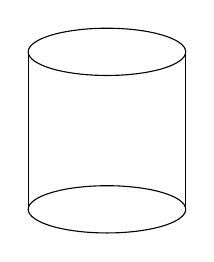
\begin{tikzpicture}
			\draw (0,0) ellipse (1 and 0.3);
			\draw (-1,0) -- (-1,-2);
			\draw (1,0) -- (1,-2);
			\draw (0,-2) ellipse (1 and 0.3);
		\end{tikzpicture}
		\caption*{Cilindro}
	\end{subfigure}
	\begin{subfigure}{0.3\textwidth}
		\centering
		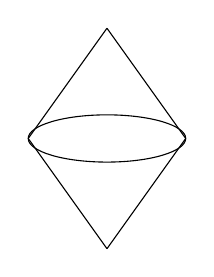
\begin{tikzpicture}
			\draw (0,-1) ellipse (1 and 0.3);
			\draw (0,0.4) -- (-1,-1);
			\draw (0,0.4) -- (1,-1);
			\draw (0,-2.4) -- (-1,-1);
			\draw (0,-2.4) -- (1,-1);
		\end{tikzpicture}
		\caption*{Suspensión}
	\end{subfigure}
	\begin{subfigure}{0.3\textwidth}
		\centering
		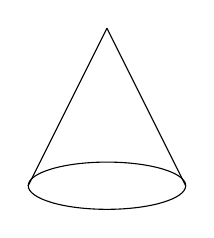
\begin{tikzpicture}
			\draw (0,0) -- (-1,-2);
			\draw (0,0) -- (1,-2);
			\draw (0,-2) ellipse (1 and 0.3);
		\end{tikzpicture}
		\caption*{Cono}
	\end{subfigure}
	\end{figure}
	\label{fsusp}Y también es posible definir la \textbf{suspensión de una función} $f:X\to Y$, que es de la forma $Sf:SX\to SY$ simplemente tomando el cociente de $f\times Id:X\times I\to Y\times I$.
	\end{defn}
	\begin{teo}
		El cono y la suspensión de un espacio complejo CW son complejos CW.
	\end{teo}
\subsection{Complejos CW para Lee (extra)}
Veamos cómo define Lee los complejos CW en su libro Introduction to Topological Manifolds:
\begin{defn}
	Si $X$ un espacio topológico no vacío, una \textbf{descomposición celular} de $X$ es una partición $\mathcal{E}$ de $X$ en subespacios que son células abiertas de manera que para cada $e\in\mathcal{E}$ de dimensión $n\geq1$ existe una \textbf{función característica} $\phi$ de una $n$-célula cerrada $D$ a $X$ que se restringe a un homeomorfismo de $\text{Int}D$ en $e$ y manda $\partial D$ en la unión de células en $\mathcal{E}$ de dimensión menor estricta que $n$.
	
	Un \textbf{complejo celular} es un espacio Housdorff $X$ junto con una descomposición celular.
\end{defn}
\begin{obs}
	Las células, aunque son homeomorfas a discos abiertos, no tienen por qué ser abiertos de $X$.
\end{obs}
\begin{defn}
	Un \textbf{complejo CW} es un complejo celular $(X,\mathcal{E})$ tal que:
	\begin{enumerate}
		\item[\textbf{C}] \textbf{(Closure finiteness)} La cerradura de cada célula intersecta a una cantidad finita de células de $X$.
		\item[\textbf{W}] \textbf{(Weak topology)} La topología de $X$ es coherente con la familia de subespacios cerrados $\{\bar{e}:e\in\mathcal{E}\}$, es decir, $U\subseteq X$ es cerrado en $X$ si y sólo si $U\cap \bar{e}$ es cerrado para cada $e\in\mathcal{E}$.
	\end{enumerate}
	Una equivalencia entre esta definición y la de Hatcher cuando $X$ es Housdorff está en el apéndice de Hatcher.
\end{defn}
\section{La homología singular de un complejo CW}
	\begin{lema}\leavevmode
	\begin{itemize}
		\item Si las $n$-celulas están indexadas por el conjunto $I_n$, \[H_k(X^n,X^{n-1})=\begin{cases}0\qquad\quad\qquad\text{si }k\neq0\\
			\bigoplus_{\alpha\in I_n}R\qquad \text{si } k=n
		\end{cases}\]
		\begin{proof}
			$H_k=\tilde H_k(X^n/X^{n-1})=\tilde H_k(\bigvee_{\alpha \in I_n}S^n)=\bigoplus_{\alpha\in I_n}H_k(S^n)$
		\end{proof}
		\item $H_k(X^n)=0$ para toda $k>n$. 
		
		Nuevamente, la homología, lo que aclance a ver la homología, lo ve solamente hasta la dimensión del espacio
		\item La inclusión $X^n\hookrightarrow X$ induce un isomorfismo $H_k(X^n)\to H_k(X)\qquad k>n$.
		
		Aquí la idea es que adjuntar células de dimensión mayor que la homología que estamos calculando no cambia la homología. Es decir, para $n>k$ se tiene que $H_k(X\cup D^n)=H_k(X)$.
	\end{itemize}
	\end{lema}
	\begin{proof}
		Fijémonos en $(X^n,X^{n-1})$, hay una sucesión exacta corta de la pareja:
		\[\begin{tikzcd}[column sep=small]
			H_{k+1}(X^n,X^{n-1}) \arrow[r] & H_k(X^{n-1}) \arrow[r] & H_k(X^n) \arrow[r] & H_k(X^n,X^{n-1})
		\end{tikzcd}\]
		Usando el inciso 1, si $k\neq n,n-1$ entonces $H_k(X^{n-1})\cong H_k(X^n)$.
		
		Bueno para demostrar (2), justamente tenemos $k>n$ y entonces resultará, fijando $k$ y bajando uno por uno, $H_k(X^n)\cong H_k(X^0)$ que es un espacio discreto y la homología de grado mayor que cero en espacios discretos es cero. Terminamos el inciso (2).
		
		Para (3), si $k<n<n+1<n+2<...$, simplemente tenemos que
		\[H_k(X^n)\cong H_k(X^{n+1})\cong...\cong H_k(X^{n+m})\]
		y si pedimos que $X$ sea de dimensión finita entonces terminaremos en algún punto y listo. El caso de dimensión infinita queda para el futuro.
	\end{proof}
\section{Homología celular}
	A continuación construimos un nuevo tipo de homología para complejos CW:
	\begin{defn} Consideremos
		\[\begin{tikzcd}[column sep=tiny]
			& H_{n-1}(X^{n-1}) \arrow[rd, "j_{n-1}"] \\
			H_n(X^n, X^{n-1}) \arrow[ru, "\partial_n"] \arrow[rr, "d_n"] && H_{n-1}(X^{n-1}, X^{n-2}) \arrow[rd, "\partial_{n-1}"] \arrow[rr, "d_{n-1}"] && H_{n-2}(X^{n-2}, X^{n-3}) \\
			& && H_{n-2}(X^{n-2}) \arrow[ru, "j_{n-2}"]
		\end{tikzcd}\]
		Resultará que las flechas horizontales que definimos con los triangulitos, es decir las $d_i$, satisfacen que \[d_{n+1}\circ d_n=0\] así que podemos bautizar el \textbf{complejo de cadenas celular} $C_\bullet^{CW}(X,R)$. Y ahora podemos definir la \textbf{homología celular}: \[H^{CW}_n(X;R)=H_n(C_\bullet^{CW}(X))\]
	\end{defn}
	\begin{teo}
		\[H_n^{CW}(X;R)\cong H_n(X;R)\qquad\forall n\geq0\]
	\end{teo}
	El primero depende de la estructura celular del espacio $X$, pero el segundo no. Así, la homología de un complejo $CW$ es independiente de la estructura celular.
	\begin{obs}\label{obs1}
		Estos grupos $H_n(X^n,X^{n-1})$ son las sumas directas de $R$, uno por cada $n$-célula de $X$.
	\end{obs}
	\begin{prop}[Consecuencias de la definición] Tomemos $X$ un complejo CW y $R=\Z$.
		\begin{enumerate}
			\item $H_n(X)=0$ si $X$ no tiene $n$-células.
			\item Supongamos que $X$ tiene exactamente $k$ $n$-céulas. Entonces $H_n(X)$ está generado por a lo más $k$ elementos, pues, como $H_n(X^n,X^{n-1})$ es abeliano libre en $n$ elementos, también lo son el subgrupo $\ker d_n$ y $\ker d_n/\img d_{n-1}=H_n(X)$.
			\item Si $X$ no tiene células de dimensiones adyacentes, entonces $H_n(X)$ es libre para todo $n$ de rango el número de $n$-células.
		\end{enumerate}
	\end{prop}
\section{Una fórmula para el homomorfismo frontera}
	Bueno, ahora tratemos de entender cómo es la $d$. Consideremos sl siguiente diagrama:
	\[\begin{tikzcd}
ed, "\varphi_{\alpha\beta}"] & X^{n-1} \arrow[d] \\
		& S^{n-1}_\beta & \bigvee_{\gamma\in I_n}S^{n-1}_\gamma = X^{n-1}/X^{n-2} \arrow[l]
	\end{tikzcd}\]
	Esta función que descubrimos $\varphi_{\alpha\beta}$ es una función entre esferas que tiene un grado $d_{\alpha\beta}$.
	\begin{teo}
		Para $n\geq 2$, el homomorfismo $d_n$ manda $e^{n}_\alpha\mapsto\sum d_{\alpha\beta}e^{n-1}_\beta$.
	\end{teo}
	\section{Ejemplos}
	\begin{ejem}
		Calculamos de dos maneras distintas la homología de $X=\bigvee_{\alpha\in I}S_\alpha^1$, por un lado usando directamente que $H_0(X)=R$ y otro usando el teorema anterior. Para el teorema anterior, descubrimos que para como sólo hay una 0-célula, para cualquier $\alpha$, $e_\alpha^1\mapsto x_0-x_0=0$, así que de hecho $d_1=0$. Resulta que $H_1=\bigoplus_IR$.
	\end{ejem}
	De hecho, esto es cierto en general:
	\begin{lema}
		Si $X$ es un complejo con una única 0-célula, entonces $d_1=0$.
	\end{lema}
	\begin{ejem}[El toro]\label{ejem:toroCW}
		Sabemos que hay una descomposición del toro como complejo CW en una 0-celda, dos 1-celdas y una 2-celda. Esto nos el siguiente complejo de cadenas:
		\[\begin{tikzcd}
			0\arrow[r]&\Z\arrow[r,"d_2"]&\Z\oplus\Z\arrow[r,"d_1=0"]&\Z\arrow[r]&0
		\end{tikzcd}\]
		Sabemos que $d_1=0$ porque sólo hay una 0-celda. Para descubrir cómo actúa $d_2$ echemos un vistazo al siguiente diagrama:
	\[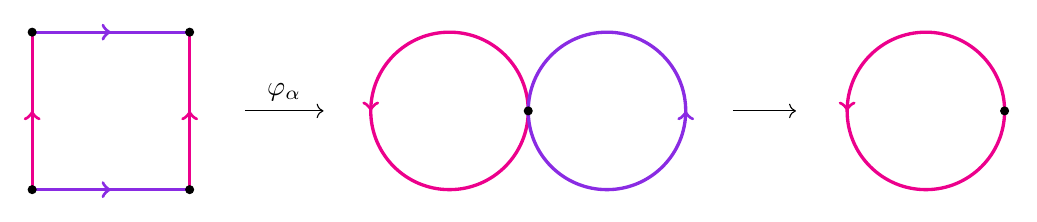
\begin{tikzpicture}[decoration={
			markings,
			mark=at position 0.5 with {\arrow{to}}
		}]
		% Sides as arrows with arrowheads in the middle
		\draw[magenta,very thick,postaction={decorate}] (0,0) -- (0,2);
		\draw[blue-violet,very thick,postaction={decorate}] (0,2) -- (2,2);
		\draw[magenta,very thick,postaction={decorate}] (2,0) -- (2,2);
		\draw[blue-violet,very thick,postaction={decorate}] (0,0) -- (2,0);

		% Vertices
		\filldraw (2,0) circle (0.05);
		\filldraw (2,2) circle (0.05);
		\filldraw (0,2) circle (0.05);
		\filldraw (0,0) circle (0.05);
		
		\draw[->] (2.7,1) -- (3.7,1) node[midway, above] {$\varphi_\alpha$};
		
		\draw[magenta,very thick,postaction={decorate}] (5.3,1) circle (1);
		\draw[blue-violet,very thick,postaction={decorate}] (7.3,1) circle (-1);
		\filldraw (6.3,1) circle (0.05);
		
		\draw[->] (8.9,1) -- (9.7,1);
		
		\draw[magenta,very thick,postaction={decorate}] (11.35,1) circle (1);
		\filldraw (12.35,1) circle (0.05);
	
	\end{tikzpicture}\]
	La frontera de la 2-celda, $S^1$ va a dar mediante la función de pegado a la cuña de dos círculos, y \textbf{recorre cada uno dos veces y en direcciones contrarias}. El cociente $X^1/X^0$ no hace nada, pues de por sí $X^0$ ya era sólo un punto, y en el último, paso, al escoger uno de los dos círculos en la cuña, nos damos cuenta de nuestra función lo recorre \textbf{de ida y luego de regreso}. Esta función es homotópica a una constante, así que es de grado cero. Al hacer esto para los dos círculos, concluimos que, $d_2=0$. Luego, $H_1(T^2)=\Z\oplus\Z$ y $H_2(T^2)=\Z$.
	\end{ejem}
	\begin{teo}[Extra]
		Una superficie compacta y conexa sólo puede ser una esfera, un toro, una suma conexa de toros, el plano proyectivo o una suma conexa de planos proyectivos.
	\end{teo}
	\begin{ejem}[El toro de género $g$]
		Resulta que el toro doble se puede ver como el cociente de un octágono identificando aristas. Y en general, el $g$-toro es el cociente de un $4g$-ágono. El resultado final es que $H_0(S_g)=\Z, H_1(S_g)=\Z^{2g}$ y $H_2(S_g)=\Z$.
	\end{ejem}
	\begin{ejem}[El plano proyectivo]
	Recordemos la descomposición más sencilla del plano proyectivo con un célula de cada dimensión:
	\[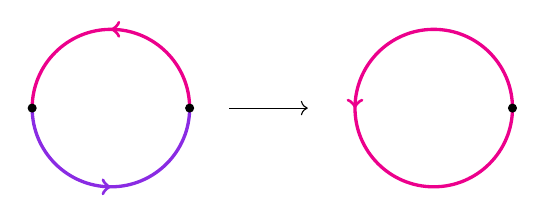
\begin{tikzpicture}[decoration={
			markings,
			mark=at position 0.5 with {\arrow{to}}
		}]
		\draw[very thick, magenta, postaction={decorate}] (0,0) arc[start angle=0, end angle=180, radius=1];
		\draw[very thick, blue-violet, postaction={decorate}] (-2,0) arc[start angle=180, end angle=360, radius=1];
		
		\filldraw (0,0) circle (0.05);
		\filldraw (-2,0) circle (0.05);
		\draw[->] (0.5,0) -- (1.5,0);
		
		\draw[magenta,very thick,postaction={decorate}] (3.1,0) circle (1);
		
		\filldraw (4.1,0) circle (0.05);

	\end{tikzpicture}\]
	Aquí, 
	\[\begin{tikzcd}
		0\arrow[r]&\Z\arrow[r,"d_2"]&\Z\arrow[r,"d_1=0"]&\Z\arrow[r]&0
	\end{tikzcd}\]
	Formalmente, para descubrir cómo actúa la función de pegado hacemos el siguiente razonamiento usando el \hyperref[subsec:grloc]{grado local}. La función que tenemos el dibujo envía el hemisferio norte (sin su frontera) en el círculo de la derecha sin el punto. La restricción de la función al hemisferio norte no ayuda a descomponer la función para calcular el grado. Como la restricción es un homeomorfismo, el grado local aquí es 1.
	
	Lo mismo sucede para el pedazo de la función en el hemisferio sur. La observación clave es que cada una de estas funciones locales se obtiene de la otra al componer con la función antípoda, que tiene grado $1$ en $S^1$. El grado de la función completa es la suma de los grados locales, así que el grado es 2. Y como sólo hay una célula de cada dimensión, $d_2=2$. Luego, $H_2(\R P^2)=0$ y $H_1(\R P^2)=\Z/2$.

	\end{ejem}
	\begin{ejem}[$\R P^n$]
		Sólo debemos generalizar el ejemplo anterior. La descomposición de $\R P^n$ como complejo $CW$ es $\R P^n=e_0\cup e_1\cup...\cup e_n$. El diagrama de arriba se vuelve:
		\[\begin{tikzcd}
			& S^{k-1} \arrow[r, "\varphi_\alpha"] \arrow[d, dashed,swap, "\bar\varphi"] & \mathbb{R}P^{k-1} \arrow[d, "q"] \\
			& S^{k-1} & \mathbb{R}P^{k-1}/\mathbb{R}P^{k-2} \arrow[l]
		\end{tikzcd}\]
		Las funciones de pegado $\varphi_\alpha$ son la proyección al cociente función antipodal en la esfera (el cubriente del plano proyectivo). Estas funciones son dos a dos, y esto hace que el hemisferio norte de $S^{k-1}$ se mapee homeomorfamente a $S^{k-1}$ menos un punto, justo como en el caso de dimesión 2.
		
		Como dijimos, las funciones que obtenemos cuando restringimos $\bar\varphi$ a cada hemisferio difieren una de la otra por el mapeo antipodal. A la hora de calcular el grado, obtenemos la fórmula $\deg (\bar{\varphi})=1+(-1)^k$.
		
		Luego,
		\[d_k=\begin{cases}2\quad\text{si }k\text{ es par}\\0\quad\text{si }k\text{ es impar}\end{cases}\]
		Esto genera la homología siguiente:
		\[\begin{tikzcd}[column sep=small]
			0 \arrow[r] & \mathbb{Z} \arrow[r, "0"] & \mathbb{Z} \arrow[r, "2"] & \cdots \arrow[r, "2"] & \mathbb{Z} \arrow[r, "0"] & \mathbb{Z} \arrow[r, "2"] & \mathbb{Z} \arrow[r, "0"] & \mathbb{Z} \arrow[r] & 0
		\end{tikzcd}\qquad\text{para }n\text{ impar}\]
		\[\begin{tikzcd}[column sep=small]
			0 \arrow[r] & \mathbb{Z} \arrow[r, "2"] & \mathbb{Z} \arrow[r, "2"] & \cdots \arrow[r, "2"] & \mathbb{Z} \arrow[r, "0"] & \mathbb{Z} \arrow[r, "2"] & \mathbb{Z} \arrow[r, "0"] & \mathbb{Z} \arrow[r] & 0
		\end{tikzcd}\qquad\quad\text{para }n\text{ par}
		\]
		Así que $H_0(\R P^n)=\Z$, $H_k(\R P^n)=\Z/2$ para $k<n$ impar,  y $H_n(\R P^n)$ es $0$ si $n$ es par, y $\Z$ si $n$ es impar.
	\end{ejem}
	\begin{ejem}[Primer ejemplo donde cambian las cosas si cambiamos de anillo]
		Tomemos $\R P^n$ y el anillo $R=\Q$.
		\[\begin{tikzcd}
			0 \arrow[r] & \mathbb{Q} \arrow[r, "0"] & \mathbb{Q} \arrow[r, "2"] & \cdots \arrow[r, "2"] & \mathbb{Q} \arrow[r, "0"] & \mathbb{Q} \arrow[r, "2"] & \mathbb{Q} \arrow[r, "d_1=0"] & \mathbb{Q} \arrow[r] & 0
		\end{tikzcd}\]
		Pero ahora la función multiplicar por 2 manda $\Q$ en todo $\Q$, algo que no pasaba con $\Z$. Esto hace que la homología sea trivial, es decir, $H_n(\R P^n,\Q)=0$ para toda $n\geq1$.
	\end{ejem}
	\begin{ejem}
		¿Y si tomamos $R=\Z/2$? Multiplicar por 2 es la función 0, así que $H_m(\R P^n,\Z/2)=\Z/2$ para $0\leq m\leq n$.
	\end{ejem}
	\begin{ejem}[La banda de Möbius]
		Tomemos la siguiente descomposición de la banda de Möbius:
		\[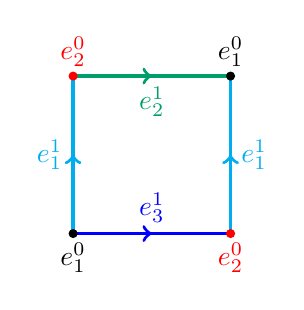
\begin{tikzpicture}[decoration={
			markings,
			mark=at position 0.5 with {\arrow{to}}
		}]
		% Sides as arrows with arrowheads in the middle
		\draw[cyan,very thick,postaction={decorate}] (0,0) -- (0,2) node[midway,left] {$e^1_1$};
		\draw[green(ncs),very thick,postaction={decorate}] (0,2) -- (2,2) node[midway, below] {$e^1_2$};
		\draw[cyan,very thick,postaction={decorate}] (2,0) -- (2,2) node[midway, right] {$e^1_1$};
		\draw[blue,very thick,postaction={decorate}] (0,0) -- (2,0) node[midway,above] {$e^1_3$};
		
		% Vertices
		\filldraw[red] (2,0) circle (0.05) node[below] {$e^0_2$};;
		\filldraw (2,2) circle (0.05) node[above] {$e^0_1$};
		\filldraw[red] (0,2) circle (0.05) node[above] {$e^0_2$};
		\filldraw (0,0) circle (0.05) node[below] {$e^0_1$};
	\end{tikzpicture}\]
	Que corresponde al complejo de cadenas
	\[\begin{tikzcd}
		0\arrow[r]&\Z\arrow[r,"d_2"]&\Z^3\arrow[r,"d_1"]&\Z^2\arrow[r]&0
	\end{tikzcd}\]
	En este caso $d_1$ no es automáticamente cero porque tenemos dos 0-celdas. Sin embargo, sabemos que la banda es conexa, así que $H_0\approx\Z$.
	
	Podemos hacer el cálculo de $d_1$ explícito (lo necesitamos para calcular $H_1(M)$) porque sabemos que se comporta exactamente como la frontera de la homología simplicial. De acuerdo a los nombres en el diagrama, podemos simplemente ver que
	\begin{equation*}
	\begin{array}{c@{\hspace{2cm}}c@{\hspace{2cm}}c}
		d_1(e^1_1)=e^0_2-e^0_1&d_1(e^1_2)=e^0_1-e^0_2&d_1(e^1_3)=e^0_2-e^0_1
	\end{array}
	\end{equation*}
	Equivalentemente,
	\begin{equation*}
	\begin{array}{c@{\hspace{2cm}}c@{\hspace{2cm}}c}
		(1,0,0)\overset{d_1}{\mapsto}(-1,1)&(0,1,0)\overset{d_1}{\mapsto}(1,-1)&
		(0,0,1)\overset{d_1}{\mapsto}(-1,1)
	\end{array}
	\end{equation*}
	Así que $\img d_1\approx \Z$, como esperábamos, y $\ker d_1\approx \langle (1,1,0),(0,1,1)\rangle\approx \Z\oplus\Z$.
	
	Para calcular $d_2$, notemos que la 2-celda está pegada sólo a lo largo de las aristas $e^1_2$ y $e^1_3$. Al colapsar el 0-esqueleto obtenemos la cuña de tres círculos, uno por cada arista. Las funciones inducidas en nuestro diagrama conmutativo son de grado 0 para $e^1_1$ y 1 para $e^1_2$ y $e^1_3$, así que $d_2(e^2)=0\cdot e^1_1+e^1_2+e^1_3$, o bien, $1\overset{d_2}{\mapsto}(0,1,1)$, de manera que $\img d_2\approx \Z$ y $\ker d_2\approx 0$. Luego, $H_1(M)\approx (\Z\oplus\Z)/\Z\approx \Z$ y $H_2(M)\approx 0$.
\end{ejem}
\section{Característica de Euler}
	Sea $Y$ un complejo $CW$ finito (con un número finito de células). De hecho esta propiedad es equivalente a que el espacio $Y$ sea compacto. Definimos la característica de Euler como
	\begin{align*}
		\chi(Y)&=(\#\text{ 0-células})-(\#\text{ 1-células})+(\#\text{ 2-células})-...\\
		&=\sum_{i=0}^\infty(-1)^i(\#\text{ }i\text{-células})\in\Z
	\end{align*}
	\begin{ejems}\leavevmode
		
		\begin{itemize}
			\item $\chi(S^n)=\begin{cases}0\qquad n\quad\text{ impar}\\2\qquad n\quad\text{ par}\end{cases}$
			\item $\chi(S^n)=\begin{cases}0\qquad n\quad\text{ impar}\\2\qquad n\quad\text{ par}\end{cases}$
			\item $\chi(\bigvee_{i=0}^nS^1)=1-n$
			\item $\chi(S_g)=1-2g+1=2-2g$
		\end{itemize}
	\end{ejems}
	\begin{teo}
		Sean $X,Y$ complejos $CW$-finitos Si $X\simeq Y$ entonces $\chi(X)=\chi(Y)$.
	\end{teo}
	\begin{prop}
		 Sea $Y$ un complejo $CW$ finito. Entonces,
		 \[\chi(Y)=\sum_{i=0}^\infty(-1)^i\ran H_i(Y;\Z)\]
		 Para entender qué es $\ran H_i$, notemos que el complejo de cadenas está hecho por grupos abelianos finitamente generados, ya que $Y$ es finito. De hecho, la homología de $Y$ es una sucesión exacta de grupos finitos finitamente generados. Luego, por el teorema de clasificación de grupos abelianos finitamente generados podemos descomponer un grupo en una expresión de la forma
		 \[A=\underbrace{\bigoplus_{i=1}^r\Z}_\text{libre de torsión}\oplus\underbrace{\text{finito}}_{\text{torsión}}\]
		 donde $r=\ran(A)$ es el rango del grupo. Éste es el número que aparece en la proposición.
	\end{prop}
	\begin{ejer}
		Sea $0\to A\to B\to C\to 0$ una sucesión exacta de grupos abelianos finitamente generados. Entonces $\text{ran }B=\text{ran }A+\text{ran }C$. (Ver \hyperref[subsec:splitting]{splitting lemma}).
	\end{ejer}
	Ahora demostremos la proposición:
	\begin{proof}
		Tomemos el complejo de cadenas celular
		\[\begin{tikzcd}[column sep=small]
			0 \arrow[r] & C_k \arrow[r, "d_k"] & C_{k-1} \arrow[r, "d_{k-1}"] & \cdots \arrow[r, "d_2"] & C_1 \arrow[r, "d_1"] & C_0 \arrow[r] & 0
		\end{tikzcd}\]
		y recordemos que $Z_n=\ker d_n$ y $B_n=\text{img }d_{n+1}$ y $H_n=Z_n/B_n$. Así que tenemos las sucesiones exactas cortas
		\[\begin{tikzcd}[column sep=small,row sep=tiny]
			0\arrow[r]&Z_n\arrow[hook,r]&C_n\arrow[r,"d_n"]&B_{n-1}\arrow[r]&0\\
			0\arrow[r]&B_n\arrow[r,hook]&Z_n\arrow[r]&H_n\arrow[r]&0
		\end{tikzcd}\]
		Usando el ejercicio, tenemos que
		\begin{align*}
			\text{ran }C_n=\text{ran }Z_n+\text{ran }B_{n-1}\\
			\text{ran }Z_n=\text{ran }B_n+\text{ran }H_{n}
		\end{align*}
		Ahora primero por definición y luego usando lo anterior,
		\begin{align*}\chi(Y)=&\sum_{i=0}^\infty(-1)^i\text{ran }C_i\\
			=&\sum_{i=0}^\infty(-1)^i\Big(\text{ran }B_i+\text{ran }H_i+\text{ran }B_{i-1}\Big)\\
			=&\sum_{i=0}^\infty(-1)^i\text{ran }H_i\qquad\qquad\square
		\end{align*}
		Nomás checando bien qué onda con $i=0$ para $\ran B_{i-1}$.
	\end{proof}
	Y con esta proposición se demuestra fácilmente el teorema de arriba.

\chapter{Homología y homotopía}	
\section{El homomorfismo de Hurewicz}
Comenzamos con algunas ideas algebraicas:

Sea $G$ un grupo y sean $g,h\in G$. El conmutador de estos elementos es $[g,h]=ghg^{-1}h^{-1}$. Dos elementos conmutan si y sólo si el conmutador es trivial. El subgrupo \textbf{derivado} o \textbf{subgrupo conmutador} es:
\[G'=\langle[g,h]|g,h\in G\rangle\leq G\]
Ahora notemos que un homomorfismo de $G$ se restringe a un homomorfismo de $G'$. Es decir, la restricción es un automorfismo de $G'$. Decimos que $G'$ es un \textbf{subgrupo característico}. Luego, esto implica que es un subgrupo normal así que hago el cociente, y resultará ser un grupo abeliano porque todo lo que no conmuta se identificó. Este grupo es $G^{\text{ab}}:=G/G'$ y se llama la \textbf{abelianización }de $G$.
\begin{obs}
	Al hacer esto con un grupo simple, cuyos subgrupos normales son él y el trivial, el cociente $G/G'$ es el grupo trivial. Pero bueno, en general la idea es producir un grupo abeliano con cualquier grupo.
\end{obs}
\begin{prop}
	Sean $G$ un grupo y $A$ un grupo abeliano. Si $\varphi:G\to A$ es un homomorfismo, entonces $\exists! \bar\varphi:G^\text{ab}\to A$ tal que 
	\[
	\begin{tikzcd}
		G \arrow[r, "\varphi"] \arrow[dr] & A \\
		& G^{\text{ab}} \arrow[u, swap, "\varphi"]
	\end{tikzcd}
	\]
	conmuta.
\end{prop}
\begin{defn}
	El \textbf{homomorfismo de Hurewicz} es
	\begin{align*}
		h:\pi_1(X,x_0)&\to H_1(X)\\
		[f]&\mapsto [f]
	\end{align*}
	que está bien definido porque en efecto los lazos son ciclos (y no depende del representante).
\end{defn}
\begin{teo}
	Si $X$ es arco-conexo, $h$ es suprayectivo y además $\ker h=\big(\pi_1(X,x_0)\big)'$. Es decir, el abelianizado del grupo fundamental es isomorfo al primer grupo de homología de $X$.
\end{teo}
\begin{coro}\leavevmode
	\begin{itemize}
		\item $\Z\cong\pi_1(S^1,x_0)\cong H_1(S^1)$
		\item $\Z\cong\pi_1(S^1,x_0)\cong H_1(S^1)$
		\item También se puede deducir para el toro que $H_1(T)\cong \Z^2$.
	\end{itemize}
\end{coro}

\section{Grupos de homotopía superiores}
	Recordemos que el grupo fundamental quedó definido como
	\begin{align*}
		\pi_1(X,x_0)=&\{f:I\to X:f(0)=f(1)=x_0\}\Big/\simeq\text{rel }0,1\\
		=&\{f:(S^1,s_0)\to(X,x_0)\}\Big/\simeq\text{rel }s_0
	\end{align*}
	En esta segunda expresión del grupo fundamental, podemos pensar que la operación del grupo está dada por una función definida en la cuña de dos círculos ya que debemos: (1) recorrer $S^1$ al doble de velocidad y luego (2) identificar el punto base con su antípoda.
	
	Así, podemos definir para $n\geq2$
	
	\[\pi_n(X,x_0)=\{f:(S^n,s_0)\to (X,x_0)\}\Big/\simeq\text{rel }s_0\]
	
	donde la operación del grupo está definida en la cuña de dos esferas $n$-dimensionales.
	
	\begin{prop}
		Para todo $n\geq 2$ y $(X,x_0)$ espacio topológico punteado, $\pi_n(X,x_0)$ es abeliano.
	\end{prop}
	\begin{obs}
		Cada elemento de $\pi_0(X,x_0)$ representa una componente arco-conexa de $X$. ¡Pero $\pi_0(X,x_0)$ no tiene estructura de grupo!
	\end{obs}
	\begin{prop}
		 $\pi_n:\Top^*\to\Grp$ es un funtor para $n\geq1$. Es decir, está bien definido en objetos y flechas, y manda la identidad en la identidad y es asociativo.
	\end{prop}
	\begin{prop}
		Aquí también hay invarianza homotópica: si $\varphi,\psi:(X,x_0)\to(Y,y_0)$ son homotópicas, las inducidas en grupos de homotopía son la misma. En particular, si dos espacios son homotópicos vía una homotopía que preserva el punto base, entonces sus grupos de homotopía son el mismo.
	\end{prop}
	El recíproco no es cierto, hay espacios con el mismo grupo de homotopía pero que no son equivalentemente homotópicos: $\R^2$ y $S^2$ tienen el mismo grupo fundamental pero su segundo grupo de homología es diferente.
	
	El recíproco no es cierto, hay espacios con el mismo grupo de homotopía pero que no son equivalentemente homotópicos: $\R^2$ y $S^2$ tienen el mismo grupo fundamental pero su segundo grupo de homología es diferente. \hyperref[ejer:homol-homot]{Aquí} hay otro ejemplo.
	
	Ahora, si pedimos que tengan el mismo grupo de homotopía y el mismo grupo de homología, ¿serán homotópicamente equivalentes?
	
	\begin{teo}[Whitehead]
		Sean $X$, $Y$ complejos $CW$. Supongamos que $f:X\to Y$ es tal que $f_*:\pi_n(X,x_0)\to\pi_n(Y,y_0)$ es un isomorfismo para toda $n\geq0$. Entonces $f$ es una equivalencia homotópica.
	\end{teo}
	De hecho sí hay espacios cuyos grupos de homotopía son isomorfos pero los espacios no son homotópicamente equivalentes, pero en estos casos el isomorfismo no está inducido por una función entre los espacios.
	\begin{teo}
		Sea $p:(\tilde{X},\tilde{ x}_0)\to(X,x_0)$ un cubriente entre espacios conexos. Entonces, $p_*:\pi_n(\tilde{X},\tilde {x}_0)\to\pi_n(X,x_0)$ es un isomorfismo para $n\geq2$.
	\end{teo}
	\begin{proof}
		Tomamos un lazo $f:S^n\to X$ y sabemos que hay un levantamiento. Eso prueba suprayectividad. Y para ver inyectividad, al tomar un lazo en el cubriente cuya proyección es homotópica a cero, podemos de hecho levantar la homotopía y obtenemos que el lazo arriba también es homotópico al constante.
	\end{proof}
	\begin{ejem}
		Los grupos de homotopía del toro para $n\geq2$ son triviales por su cubriente universal, $\R^2$, que es contraible. En general, cualquier espacio que tenga un cubriente contraible tiene grupos de homotopía de orden superior triviales.
	\end{ejem}
		
\chapter{Ejercicios}
	\begin{ejer}
	Calcule la homología de la pareja $(X,A)$ cuando $A$ es un subconjunto finito del toro $X=S^1\times S^1$.
\end{ejer}
\begin{proof}[Solución]
	Como $C_n(A)\approx0$ para $n\geq1$, tenemos que $H_n(X,A)\approx H_n(X)$ para $n>1$.
	
	Para el caso $n=0$ primero notemos que $(X,A)$ es una buena pareja tomando la unión de vecindades disjuntos alrededor de cada punto en $A$ para hacer la retracción. Esto implica que $H_n(X,A)\approx \tilde{H}_n(X/A)$.  Luego, la homología reducida \hyperref[sec:6.4]{cumple} que $H_0(X/A)\approx\tilde{H}_0(X/A)\oplus R$, y como $X/A$ es arco-conexo, entonces $H_0(X,A)\approx0$.
	
	Para encontrar el primer grupo de homología usamos la sucesión exacta de la pareja:
	\[\begin{tikzcd}[column sep=small,row sep=tiny]
		\cdots\arrow[r]&\tilde{H}_1(A)\arrow[r]&\tilde{H}_1(X)\arrow[r]&\tilde{H}_1(X/A)\arrow[r]&\tilde{H}_0(A)\arrow[r]&\tilde{H}_0(X)\arrow[r]&\cdots\\
		\cdots\arrow[r]&0\arrow[r]&R\oplus R\arrow[r]&\tilde{H}_1(X/A)\arrow[r]&\bigoplus_{k-1}R\arrow[r]&0\arrow[r]&\cdots
	\end{tikzcd}\]
	donde $|A|=k$.
	
	Ahora invocamos el \hyperref[subsec:splitting]{splitting lemma}. Tenemos una sucesión exacta corta de grupos abelianos, y como el de hasta la derecha es libre, la sucesión se separa y $\tilde{H}_1(X/A)\approx (R\oplus R)\oplus\left(\bigoplus_{k-1}R\right)\approx \bigoplus_{k+1}R$.
\end{proof}
\begin{ejer}\label{ejer:homol-homot}Demuestre que $S^1 \times S^1$ y $S^1 \vee S^1 \vee S^2$ tienen grupos de homología (con coeficientes enteros) isomorfos pero no son homotópicamente equivalentes.
\begin{proof}[Solución]
	Por sus descomposiciones como complejos CW, sabemos que la homología de ambos espacios está dada por el complejo de cadenas
	\[\begin{tikzcd}[column sep=small]
		0\arrow[r]&\Z\arrow[r,"d_2"]&\Z^2\arrow[r,"0"]&\Z\arrow[r]&0
	\end{tikzcd}\]
	\hyperref[ejem:toroCW]{Ya hemos visto que} $d_2=0$ para el caso del toro. Ver que también es cierto para el espacio $S^1\vee S^1\times S^2$ es sencillo, ya que la función de pegado colapsa la frontera de la única 2-celda a un sólo punto, así que induce funciones de grado cero en la homología.
	
	Si estos espacios fueran homotópicamente equivalementes, entonces, \hyperref[1.2.1]{sus grupos fundamentales serían isomorfos}. Sabemos que el grupo fundamental del toro es $\Z\times\Z$, y el de $S^1 \vee S^1 \vee S^2$ es isomorfo a $\Z\ast\Z$, ya que \hyperref[sec:grp-fund-cuña]{el grupo fundamental de una cuña de espacios} es isomorfo al producto libre de sus grupos fundamentales.
\end{proof}
\end{ejer}
\begin{ejer}
	Construya una función suprayectiva $f:S^n\to S^n$ de grado 0, $n\geq1$.
\end{ejer}
	\begin{proof}[Solución]
	Como el grado de la suspensión de una función es el mismo que el de la función, y $S^{n+1}=SS^n$, basta demostrar el enunciado para $S^1$.
	
	Proponemos \href{https://folk.ntnu.no/gereonq/MA3403H2018/MA3403_Exercise04_Soln.pdf}{esta idea} para demostrar mostrar el caso $n=1$:
	
	Definir una función $g$ que sea recorrer el hemisferio sur de ida y de regreso. No es suprayectiva así que es de grado 0.
	
	Componer $g$ con $f$, donde $f(z)=z^2$. La composición es suprayectiva y su grado es el producto de los grados, 0.
\end{proof}
\begin{ejer}
	Calcule los grupos de homología del espacio obtenido de $S^2$ al identificar el polo norte y el polo sur en un sólo punto.
\end{ejer}
	\begin{proof}[Solución]
	La descomoposición más sencilla (que pude encontrar) de este espacio como complejo CW está dada así:
		\begin{itemize}
		\item Una 0-celda, que es el punto que resaltamos en el dibujo.
		\item Dos 1-celdas, que son los círculos que se tocan en el punto.
		\item Dos 2-celdas. Cada una está pegada a lo largo de las dos 1-celdas. Es como cuando pegamos dos discos a lo largo de una circunferencia para construir una esfera, pero aquí pegamos dos discos a lo largo de la cuña de dos circunferencias.
	\end{itemize}
	\[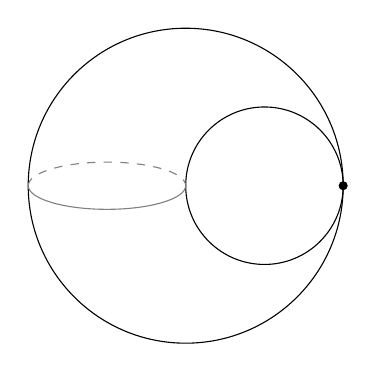
\begin{tikzpicture}
		% Outer circle
		\draw (0,0) circle (2);
		
		% Inner circle
		\draw (1,0) circle (1);
		
		%3D
		\draw[gray] (-2,0) arc (180:360:1 and 0.3);
		\draw[gray,dashed] (-2,0) arc (180:0:1 and 0.3);
		
		% Common point
		\filldraw (2,0) circle (0.05);
	\end{tikzpicture}\]
	Esto genera el siguiente complejo de cadenas:
	\[\begin{tikzcd}[column sep=small]
		0\arrow[r]&\Z^2\arrow[r,"d_2"]&\Z^2\arrow[r,"d_1"]&\Z\arrow[r]&0
	\end{tikzcd}\]
	Como sólo hay una 0-celda, sabemos que $d_1=0$. Sólo nos falta encontrar $d_2$. Para esto, tenemos el siguiente diagrama:
	\[\begin{tikzcd}[column sep=small]
		S^1_\alpha\arrow[r,"\varphi_\alpha"]\arrow[d,dashed,"\varphi_{\alpha\beta}"]&X^1=S^1\vee S^1\arrow[d]\\
		S^1_\beta&X^1/X^0=S^1\vee S^1\arrow[l]
	\end{tikzcd}\]
	¿Qué está pasando aquí? Estamos pensando que $S^1_\alpha$ es la frontera de una de las dos 2-celdas que pegamos mediante $\varphi_\alpha$. Como sólo hay una 0-celda, el cociente $X^1/X^0$ no hizo nada, y la última flecha consiste en simplemente escoger cualquier de los dos círculos son 1-celdas.
	
	El mapeo $\varphi_\alpha$ tiene la gracia de enviar la circunferencia inicial en dos circunferencias. Cuando nos quedamos con una sólo de ellas, vemos que el efecto de la composición $\varphi_{\alpha\beta}$ fue enviar $S^1_\alpha$ en $S^1_\beta$, así que es una función de grado 1. Lo mismo sucede cuando escogemos la otra circunferencia, $S^1_\gamma$. De acuerdo a nuestro teorema, tenemos que $d_2(e^2_\alpha)=1\cdot e^1_\beta+1\cdot e^1_\gamma$.
	
	Y lo mismo para la otra 2-celda. Luego,
	\begin{align*}
		d_2:\Z^2&\to\Z^2\\
		(1,0)&\mapsto (1,1)\\
		(0,1)&\mapsto (1,1)
	\end{align*}
	Así que $\img d_2\cong\Z$ y $\ker d_2\cong\langle (1,0)-(0,1)\rangle\cong\Z$, y entonces $H_2(X,\Z)\cong H_1(X,\Z)\cong H_0(X,\Z)\cong\Z$ y $H_n(X,\Z)\cong0$ para $n\geq3$.
\end{proof}
\begin{ejer}
	Calcule los grupos de homología de $S^1\times(S^1\vee S^1)$.
\end{ejer}
\begin{proof}[Solución]
	Se trata del siguiente espacio:
	\[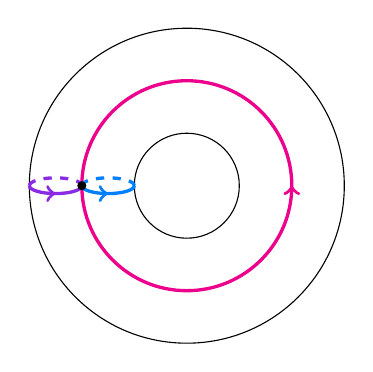
\begin{tikzpicture}[decoration={
			markings,
			mark=at position 0.5 with {\arrow{to}}
		}]
	% Outer circle
	\draw (0,0) circle (2);
	\draw[magenta,very thick,postaction={decorate}] (0,0) circle (-4/3);
	\draw (0,0) circle (2/3);
	
	%3D
	\draw[blue-violet,very thick,postaction={decorate}] (-2,0) arc (180:360:1/3 and 0.1);
	\draw[blue-violet,very thick,dashed] (-2,0) arc (180:0:1/3 and 0.1);
	\draw[azure,very thick,postaction={decorate}] (-4/3,0) arc (180:360:1/3 and 0.1);
	\draw[azure,very thick,dashed] (-4/3,0) arc (180:0:1/3 and 0.1);
	
	% Common point
	\filldraw (-4/3,0) circle (0.05);
	\end{tikzpicture}\hspace{2cm}
	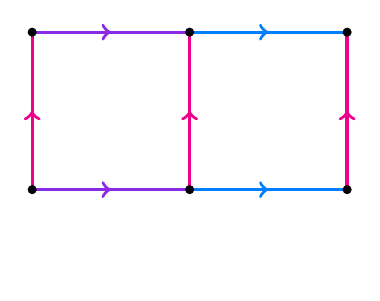
\begin{tikzpicture}[decoration={
		markings,
		mark=at position 0.5 with {\arrow{to}}
	}]
	% Sides as arrows with arrowheads in the middle
	\draw[magenta,very thick,postaction={decorate}] (0,0) -- (0,2);
	\draw[blue-violet,very thick,postaction={decorate}] (0,2) -- (2,2);
	\draw[magenta,very thick,postaction={decorate}] (2,0) -- (2,2);
	\draw[blue-violet,very thick,postaction={decorate}] (0,0) -- (2,0);
	
	\draw[magenta,very thick,postaction={decorate}] (4,0) -- (4,2);
	\draw[azure,very thick,postaction={decorate}] (2,2) -- (4,2);
	\draw[azure,very thick,postaction={decorate}] (2,0) -- (4,0);

	% Vertices
	\filldraw (2,0) circle (0.05);
	\filldraw (2,2) circle (0.05);
	\filldraw (0,2) circle (0.05);
	\filldraw (0,0) circle (0.05);
	\filldraw (4,0) circle (0.05);
	\filldraw (4,2) circle (0.05);
	
	\filldraw[white] (0,-1) circle (0.05);
	\end{tikzpicture}\]
	Cuyo complejo de cadenas celular es:
	\[\begin{tikzcd}[column sep=small]
		0\arrow[r]&\Z^2\arrow[r,"d_2"]&Z^3\arrow[r,"0"]&\Z\arrow[r]&0
	\end{tikzcd}\]
	Y por un razonamiento análogo al cálculo de la \hyperref[ejem:toroCW]{homología del toro}, $d_2=0$ y concluimos que $H_2(X)=\Z^2$, $H_1(X)=H_0(X)=\Z$.
	\end{proof}
	\begin{ejer}
	Use la sucesión de Mayer-Vietoris para calcular los grupos de homología del espacio obtenido de pegar una banda de Möbius $M$ al toro $S^1\times S^1$ vía un homeomorfismo del círculo frontera de $M$ al ecuador $S^1\times\{0\}$ del toro.
	\end{ejer}
	\begin{proof}[Solución]
		Primero recordemos las estructuras celulares que le dimos a estos espacios:
		\[
		%Toro
		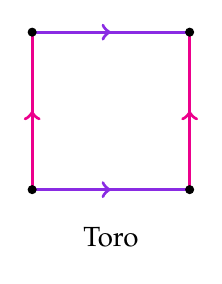
\begin{tikzpicture}[decoration={
				markings,
				mark=at position 0.5 with {\arrow{to}}
			}]
			% Sides as arrows with arrowheads in the middle
			\draw[magenta,very thick,postaction={decorate}] (0,0) -- (0,2);
			\draw[blue-violet,very thick,postaction={decorate}] (0,2) -- (2,2);
			\draw[magenta,very thick,postaction={decorate}] (2,0) -- (2,2);
			\draw[blue-violet,very thick,postaction={decorate}] (0,0) -- (2,0);
			
			% Vertices
			\filldraw (2,0) circle (0.05);
			\filldraw (2,2) circle (0.05);
			\filldraw (0,2) circle (0.05);
			\filldraw (0,0) circle (0.05);
			
			\node at (1,-.6) {Toro};
		\end{tikzpicture}\qquad\qquad\qquad
		%Banda de Möbius
		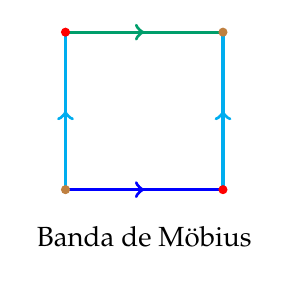
\begin{tikzpicture}[decoration={
				markings,
				mark=at position 0.5 with {\arrow{to}}
			}]
			% Sides as arrows with arrowheads in the middle
			\draw[cyan,very thick,postaction={decorate}] (0,0) -- (0,2);
			\draw[green(ncs),very thick,postaction={decorate}] (0,2) -- (2,2);
			\draw[cyan,very thick,postaction={decorate}] (2,0) -- (2,2);
			\draw[blue,very thick,postaction={decorate}] (0,0) -- (2,0);			
			% Vertices
			\filldraw[red] (2,0) circle (0.05);
			\filldraw[brown] (2,2) circle (0.05);
			\filldraw[red] (0,2) circle (0.05);
			\filldraw[brown] (0,0) circle (0.05);
			
			\node at (1,-.6) {Banda de Möbius};
		\end{tikzpicture}\]
			
%		%Espacios pegados
%		\[\begin{tikzpicture}[decoration={
%			markings,
%			mark=at position 0.5 with {\arrow{to}}
%		}]
%		% Sides as arrows with arrowheads in the middle
%		\draw[magenta,very thick,postaction={decorate}] (0,0) -- (0,2);
%		\draw[blue-violet,very thick,postaction={decorate}] (0,2) -- (2,2);
%		\draw[magenta,very thick,postaction={decorate}] (2,0) -- (2,2);
%		\draw[blue-violet,very thick,postaction={decorate}] (0,0) -- (2,0);
%		
%		\draw[magenta,very thick,postaction={decorate}] (4,0) -- (4,2);
%		\draw[azure,very thick,postaction={decorate}] (2,2) -- (4,2);
%		\draw[azure,very thick,postaction={decorate}] (2,0) -- (4,0);
%		
%		% Vertices
%		\filldraw (2,0) circle (0.05);
%		\filldraw (2,2) circle (0.05);
%		\filldraw (0,2) circle (0.05);
%		\filldraw (0,0) circle (0.05);
%		\filldraw (4,0) circle (0.05);
%		\filldraw (4,2) circle (0.05);
%		
%		\filldraw[white] (0,-1) circle (0.05);
%	\end{tikzpicture}\]
	
	No es obvio cómo pegarlos porque el círculo frontera de la banda de Möbius está formado por dos aristas (la verde y la azul fuerte), que deberían ir pegadas a una sola de las aristas del toro. Entonces, técnicamente no nos conviene usar la sucesión de Mayer-Vietoris en su versión para complejos CW. Pero esto no es problema, porque, aunque ni el toro ni la banda son abiertos de nuestro espacio, sí son retractos por deformación de ciertas vecindades.
	
	Una vez dicho esto, tenemos la sucesión exacta
	\[\begin{tikzcd}
		0 \arrow[r] & \tilde{H}_2(T\cap M) \arrow[r] & \tilde{H}_2(T)\oplus \tilde{H}_2(M) \arrow[r] & \tilde{H}_2(X) \arrow[r] & \tilde{H}_1(T\cap M)
	\end{tikzcd}\]
	\[\begin{tikzcd}
		\arrow[r]&\tilde{H}_1(T\cap M) \arrow[r,"\Phi_1"] &\tilde{H}_1(T)\oplus \tilde{H}_1(M) \arrow[r] & \tilde{H}_1(X) \arrow[r] & \tilde{H}_0(T\cap M)&&
	\end{tikzcd}\]
	
	Que, aplicando todo lo que sabemos de estos espacios, se traduce a
	
		\[\begin{tikzcd}
		0 \arrow[r] & 0 \arrow[r] & \Z \arrow[r,"\Psi_2"] & \tilde{H}_2(X) \arrow[r,"\delta_2"] & \Z
	\end{tikzcd}\]
	\[\begin{tikzcd}
		\arrow[r]&\Z \arrow[r,"\Phi_1"] &\Z\oplus \Z \oplus\Z \arrow[r,"\Psi_1"] & \tilde{H}_1(X) \arrow[r] & 0&&
	\end{tikzcd}\]
	
%	\[\begin{tikzcd}
%		0 \arrow[r] & H_2(T^2\cap M) \arrow[r,"(i_{*2}\text{,}-j_{*2})"] & H_2(T^2)\oplus H_2(M) \arrow[r,"k_{*2}+\ell_{*2}"] & H_2(X) \arrow[r,"\delta"] & H_1(T^2\cap M)\\
%		\arrow[r]&H_1(T^2\cap M) \arrow[r,"(i_{*1}\text{,}-j_{*1})"] &H_1(T^2)\oplus H_1(M) \arrow[r,"k_{*1}+\ell_{*1}"] & H_1(X) \arrow[r,"\delta"] & H_0(T^2\cap M)&&
%	\end{tikzcd}\]
	
	Creemos que basta con conocer la función $\Phi_1$ para encontrar el primer y segundo grupos de homología de $X$. Veamos:
	\begin{itemize}
		\item $\tilde{H}_2(X)/\ker\delta_2\approx\img\delta$, es decir, $\tilde{H}_2(X)/\img\Psi_2\approx\ker\Phi$. Sabemos que $\Psi_2$ es inyectiva, así que su imagen es isomorfa a $\Z$. $\tilde{H}_2(X)\Z\approx\ker\Phi_1$.
		\item $\tilde{H}_1(X)\approx\img\Psi_1\approx\Z\oplus\Z\oplus\Z/\ker\Psi_1\approx\Z\oplus\Z\oplus\Z/\img\Phi_1$.
	\end{itemize}
	Ahora recordemos: dadas las inclusiones $i:T\cap M\hookrightarrow T$ y $j:T\cap M\hookrightarrow M$, $\Phi_1=(i_*,j_*)$. La intersección de $T$ y $M$ es un ecuador del toro, y el círculo frontera de la banda de Möbius. Así, la inclusión envía un generador de la intersección en: uno de los generadores del primer grupo de homología del toro; y dos veces el generador del primer grupo de homología de la banda. En símbolos:
	\[1\overset{\Phi_1}{\mapsto}(1,0)\qquad1\overset{\Phi_1}{\mapsto}2\qquad\text{es decir,}\qquad\Phi_1(1)=(1,0,2)\]
	Así que $\ker\Phi_1=0$ y $\img\Phi_1=\Z$, así que $\tilde{H}_2(X)\approx\Z$, $\tilde{H}_1(X)\approx\Z\oplus\Z$ y desde luego $\tilde{H}_n(X)\approx0$ para $n=0$ y $n>2$.
	
	\end{proof}
	

\end{document}